\documentclass[10pt,a4paper,twocolumn]{article}
\usepackage[T1]{fontenc}
\usepackage{lmodern}
\usepackage[utf8]{inputenc}
\usepackage[a4paper,margin=1.8cm,columnsep=0.6cm]{geometry}
\usepackage{microtype}
\usepackage{amsmath,amssymb,amsthm}
\usepackage{booktabs,tabularx,array}
\usepackage[shortlabels]{enumitem}
\usepackage{xcolor}
\usepackage{listings}
\usepackage{caption}
\usepackage{tikz}
\usetikzlibrary{arrows.meta,positioning,fit,backgrounds,calc}
\usepackage[colorlinks=true,linkcolor=blue!50!black,urlcolor=blue!50!black,citecolor=blue!50!black]{hyperref}

\setlist{nosep}
\raggedbottom
\setlength{\emergencystretch}{3em}
\captionsetup{font=small,labelfont=bf}
\newtheorem{property}{Property}
\newtheorem{proposition}[property]{Proposition}
\newtheorem{definition}[property]{Definition}
\newtheorem{theorem}[property]{Theorem}
\newcolumntype{L}[1]{>{\raggedright\arraybackslash}p{#1}}
\newcommand{\code}[1]{\texttt{#1}}

\definecolor{untrusted}{RGB}{200,50,50}
\definecolor{trusted}{RGB}{40,80,180}
\definecolor{enclave}{RGB}{20,120,80}
\definecolor{chain}{RGB}{110,60,160}
\tikzset{
  box/.style={draw,rounded corners=2pt,align=center,font=\footnotesize,inner sep=4pt,minimum height=0.9cm,fill=white},
  ubox/.style={box,draw=untrusted,thick,fill=untrusted!6},
  ebox/.style={box,draw=enclave,thick,fill=enclave!7},
  cbox/.style={box,draw=chain,thick,fill=chain!6},
  gbox/.style={box,draw=gray,fill=gray!8},
  arr/.style={-{Stealth[length=2.2mm]},thick},
  darr/.style={-{Stealth[length=2.2mm]},thick,dashed},
  lbl/.style={font=\scriptsize,align=center,fill=white,inner sep=1pt},
  zone/.style={draw,dashed,rounded corners=4pt,inner sep=7pt},
}
\lstdefinelanguage{Solidity}{
  keywords={function,returns,private,if,else,require},
  sensitive=true, comment=[l]{//}}
\lstset{basicstyle=\ttfamily\footnotesize,keywordstyle=\color{trusted}\bfseries,
  commentstyle=\color{gray}\itshape,frame=single,rulecolor=\color{gray!50},
  columns=fullflexible,keepspaces=true,breaklines=true,xleftmargin=0.5em,xrightmargin=0.5em}


\title{\Large\textbf{A Payment Firewall for AI Agents:\\ Bounded Spending Under Agent Compromise, and What Refunds Leak}}
\author{Adarsh Kumar\\ Department of Electrical Engineering\\ Indian Institute of Technology Patna\\ \small\texttt{adarsh\_2501ec16@iitp.ac.in}}
\date{November 2026}

\newcommand{\baseConfidentialCalls}{20}
\newcommand{\baseConfidentialMedian}{21.6}
\newcommand{\basePlainCalls}{20}
\newcommand{\basePlainMedian}{2.0}
\newcommand{\basePlaintextCalls}{20}
\newcommand{\basePlaintextMedian}{6.7}
\newcommand{\baseRuns}{2}
\newcommand{\baselinesCaption}{2 runs of 10 interleaved rounds each.}
\newcommand{\benchCaption}{Local signer: 2 runs on separate goals, 100 calls, every one reported (approved: paid 60; rejected: policy-rejected 40). Signer in the enclave: one run, 50 calls, every one reported (approved: failed 1; approved: paid 29; rejected: policy-rejected 20).}
\newcommand{\fundingcheck}{30}
\newcommand{\fundingmax}{23.8}
\newcommand{\fundingmedian}{19.4}
\newcommand{\fundingn}{20}


\begin{document}
\maketitle

\begin{abstract}
AI agents are beginning to pay for the services they use: under x402, an agent answers an HTTP 402 response with a signed stablecoin
authorization. It decides what to buy by reading text written by the party it pays, and in the common design the same process holds the key.
We ask what spending authority survives when that process is fully compromised. In our design the agent can only request a payment. A contract
holds the user's budget and per-call cap, and a signer accepts only a goal and a sequence number and signs a payment that only x402's
auth-capture escrow can collect, with the contract as operator, so every payment passes the contract's checks on the canonical chain. The payer is
derived for the user's wallet, and a goal opens only with the signer's statement saying so. For a goal with an honest setup and signer we prove,
over an explicit transition model, that lifetime vendor payments total at most min(budget, cap $\times$ calls), whatever the agent does and whatever
the signer's RPC reports; 262,144 fuzzed transitions against the deployed escrow's code and a live campaign of 29 attack strategies, with the
signer in an Intel TDX enclave, found no violation. Encrypting the limits (Inco Lightning) buys less than it seems. Refunds of unpaid approvals made the
policy free to probe; a public attempt budget bounds the decision channel to $m$ bits, yet on realistic caps a vendor with five probes prices within 4\% of
the cap. In matched runs on Base Sepolia a paid call took a median of 2.0\,s with plain x402, 6.7\,s with plaintext on-chain limits and 21.6\,s with
encrypted ones. We also specify a key-release protocol for digital goods whose dispute predicate the contract decides itself.
\end{abstract}

\section{Introduction}

Language-model agents increasingly act on the web on a user's behalf: they search, call APIs and
assemble results. Paying for those calls has required accounts, cards and invoices that an
autonomous agent cannot hold. The x402 protocol~\cite{x402} removes that barrier. A server answers a
request with HTTP status 402 and a machine-readable price, the client returns a signed stablecoin
authorization~\cite{eip3009}, and settlement on a blockchain takes seconds.

An agent that buys this way must do two things. It must read what the seller sends (price, payee and
a free-text description) to decide whether a purchase serves its goal, and it must then produce a
payment. In the common design both happen in one process, and that process holds the signing
key. This is where \emph{indirect prompt injection}~\cite{greshake2023} does the most damage: text a
seller places in its own description can steer the agent, and a steered agent with a payment key
moves money that cannot be recovered. A 2026 code review, summarised by the Cloud Security
Alliance~\cite{csa2026}, reported that default x402 clients applied no spending limit until fixes in
August 2026, and the per-payment cap those fixes added can be switched off by a flag.

Separating the model's reasoning from spending authority is not new. CaMeL~\cite{camel} checks
capability policies outside the model that reads untrusted data, and PACE~\cite{pace} has a verifier
sign each transaction a smart account will execute. We take that separation as given and ask a
narrower question: when the agent's process is fully compromised, what spending authority does it keep
over the life of a goal, and what does it learn about the user's limits? Answering it for x402 turned
up three problems that a design for this setting has to solve, and they organise this paper.

The first is that a signature outlives the approval behind it. An EIP-3009 transfer signed for an
approved request can be collected whatever later happens to the approval, so the signer must be right
about the chain: a lying RPC endpoint, or an approval on a block that is later dropped, becomes money.
We remove that dependence by signing only payments that x402's auth-capture escrow can collect, with
the policy contract as the escrow's operator, so the contract's own checks run on the canonical chain
when money moves (Section~\ref{sec:escrow}). The second is setup. The user funds an address that
reaches the console through the agent's process, so a compromised agent can name an address it holds.
The payer is now derived for the user's wallet inside the signer, and a goal opens only with the
signer's statement saying so (Section~\ref{sec:enrollment}). The third is leakage. Refunding an approval
that was never paid is necessary for accounting and makes the policy free to question: a request that
consumes nothing still has its decision published. A private policy then needs a separate budget of
questions, and even with one, the private limit protects less than its encryption suggests
(Section~\ref{sec:leakeval}).

\paragraph{Contributions.}
\begin{enumerate}
  \item \emph{Escrow-gated authorization with authenticated setup, and a lifetime spending bound.}
        Under an adversary with arbitrary code execution in the agent, on a goal whose setup and
        signer are honest, vendor payments over the goal's life total at most
        $\min(\text{budget}, \text{cap} \times \text{calls})$, to allowlisted payees only, whatever the
        signer's RPC reports. We state the bound over an explicit transition model, prove the
        invariants it rests on for every transition, and test them by stateful fuzzing against the
        deployed escrow's code, by mutation, and by a live adversary campaign
        (Sections~\ref{sec:design}--\ref{sec:security} and~\ref{sec:eval}).
  \item \emph{Refund-induced leakage.} Reclaim, which restores spending capacity to unpaid
        approvals, let an adversary binary-search the encrypted cap of our own deployed contract without
        permanently consuming budget or calls (gas, fees and time still cost). A public attempt budget bounds the decision channel to $m$ bits of average min-entropy
        leakage, under assumptions we state in the theorem. On realistic cap distributions the bound
        leaves little: a vendor with five probes prices within about 4\% of the cap
        (Sections~\ref{sec:attempts}, \ref{sec:leakthm} and~\ref{sec:leakeval}).
  \item \emph{A matched comparison.} Plain x402, the same escrow path with plaintext on-chain limits,
        and the confidential design, measured interleaved on the same network, relay and vendor; an
        enclave-held policy with on-chain rollback protection, built and measured on a fork; and an
        injection study that gives every arm the same agent interface
        (Section~\ref{sec:eval}).
\end{enumerate}

\noindent We also specify a key-release protocol for digital goods that a vendor is paid for only by
publishing the decryption key, with a dispute predicate the contract decides itself; the predicate is
built and measured, and the rest of the protocol is not (Section~\ref{sec:delivery}). The live
campaign, a benchmark and a storage-wipe test ran with the signer in an Intel TDX enclave on Oasis ROFL;
the matched baselines used a signer on a local machine (Section~\ref{sec:eval}).

\paragraph{Terms.} We keep four events apart throughout. \emph{Authorization} is the vault's approval of
a request and the signer's signature over it. \emph{Funding} moves the payer's tokens into the escrow.
\emph{Capture} pays the vendor from the escrow. \emph{Delivery} is the vendor handing over what was
bought, which nothing in the implemented system ties to capture.

\section{Background}
\label{sec:background}

\paragraph{x402 and EIP-3009.} In x402's \code{exact} scheme a server's 402 body lists the payments it
accepts: network, asset, payee, maximum amount, resource, a free-text description and
\code{maxTimeoutSeconds}, the ``maximum time allowed for payment completion''. It is a deadline for one
exchange, not a reservation. An optional Offer and Receipt extension~\cite{x402offer} lets the server sign
its terms, including an optional \textit{validUntil}. The client signs an EIP-3009~\cite{eip3009}
authorization, an EIP-712~\cite{eip712} typed message $(\mathit{from}, \mathit{to}, \mathit{value},
\mathit{validAfter}, \mathit{validBefore}, \mathit{nonce})$. A token executes each $(\mathit{from},
\mathit{nonce})$ at most once and refuses it at or after \textit{validBefore}. In
\code{transferWithAuthorization} anyone may submit the message; in \code{receiveWithAuthorization} only its
\textit{to} address may. The \code{exact} scheme also defines an ERC-7710~\cite{erc7710} delegation method
under which a smart account pays; we return to it in Section~\ref{sec:related}.

\paragraph{Auth-capture.} x402's \code{auth-capture} scheme~\cite{x402authcapture} runs on the
commerce-payments \code{AuthCaptureEscrow}~\cite{commercepayments}. A payment is a \code{PaymentInfo}
struct: operator, payer, receiver, token, maximum amount, three deadlines, fee bounds, fee receiver and a
salt. The payer signs a \code{receiveWithAuthorization} to a token collector. The escrow accepts
\code{authorize} (fund and hold), \code{charge} (fund and pay at once), \code{capture} and \code{void} only
from the struct's operator; the payer alone may \code{reclaim} a hold once its capture deadline has passed.
Section~\ref{sec:binding} gives the exact encoding and what each contract checks.

\paragraph{Inco Lightning.} Inco Lightning~\cite{inco} lets contracts on Base hold encrypted values,
represented on chain by 32-byte \emph{handles}. Users encrypt inputs on the client, and a contract converts
a ciphertext into a handle bound to the submitting address. Operations such as comparison, conjunction,
selection and subtraction return new handles at once and emit events; Inco's covalidators, running in
trusted hardware off chain, evaluate them afterwards. A contract cannot branch on an encrypted value. It
may mark a handle for public decryption, after which a threshold of covalidators signs the plaintext and
the contract verifies that signature on chain. Confidentiality and correct evaluation both rest on Inco's
covalidators and their hardware; Lightning is not homomorphic encryption.

\paragraph{Oasis ROFL and Intel TDX.} Intel TDX runs a virtual machine whose memory is protected from the
host and can be remotely attested. Oasis ROFL~\cite{rofl} runs containers in such machines under a policy
registered on the Sapphire chain, which lists the enclave measurements the application accepts, and
derives keys deterministically from the application's identity and a key identifier, releasing them only
to instances that policy admits.

\section{Threat Model and Assumptions}
\label{sec:threat}

We consider three adversaries.
\textbf{A1}, a persuasive vendor, controls everything a resource server returns, including prices, payees
and descriptions, and aims to make the agent pay more, more often, or to someone else.
\textbf{A2} has arbitrary code execution in the agent's process, the \emph{orchestrator}: it holds the relay
key, relays everything between the signer and the user's console, and may submit any request to the policy
contract and any query to the signer, in any order. A2 subsumes A1, and our claims about the agent are made
against A2. \textbf{A3}, a dishonest vendor, collects a payment after its hold has ended, or collects in
time and delivers nothing or something worthless. The implemented system addresses late funding;
non-delivery is the subject of Section~\ref{sec:delivery}.

\paragraph{What the adversaries cannot do.} Break Keccak-256 or ECDSA over secp256k1; obtain the user's
wallet key; rewrite the canonical chain. The signer's RPC endpoint may lie, and blocks may be dropped from
the chain it reads; for payment authorization after a stable, authenticated setup this costs liveness and
cannot widen the loss bound (Section~\ref{sec:escrow}). The leakage theorem makes a stronger assumption
about dropped blocks, stated in it (Section~\ref{sec:leakthm}).

\paragraph{Trusted components.} The loss bound assumes an uncompromised signer: the payer is an ordinary
key, so a compromised signer can sign a plain transfer and take the funded balance. It also trusts the
ROFL application's administrator, who can change which enclave measurements receive the application's
keys. The user's console and the user's own RPC endpoint are trusted; the console is built with the vault
address and the signer's enrollment address fixed.

\paragraph{Inco.} We separate what we assume of Inco from what we test, since a verified signature
establishes only that a threshold of covalidators endorsed a plaintext. We assume:
\begin{enumerate}[(I1)]
  \item \emph{Correct evaluation:} each handle an operation returns evaluates to that operation applied to
        the plaintexts of its inputs.
  \item \emph{Ordered evaluation and binding:} the operation graph is evaluated in the order of the
        canonical chain's transactions and events, so that the budget handle a request reads is the one
        the previous transaction wrote, and the decision handle the vault stores for $(g, s)$ is the one
        that request computed.
  \item \emph{Unforgeable attestation:} a threshold signature verifies for $(h, v)$ only if handle $h$
        evaluates to $v$.
  \item \emph{Access control:} only the vault can use the budget and cap handles as operands.
  \item \emph{Confidentiality:} no plaintext of a budget or cap handle reaches anyone; only the decisions the
        vault reveals are decrypted.
\end{enumerate}
The loss bound needs I1 to I4; the leakage theorem needs I5 as well. What this paper tests is the
contract logic \emph{given} these properties, using Inco's test double, and the live behaviour of the deployed
service in our runs; neither establishes the properties themselves. If I1 or I3 fails, the public call count,
the allowlist and the funded balance still bound the loss.

\section{Design}
\label{sec:design}

\begin{figure*}[t]
\centering
\resizebox{\linewidth}{!}{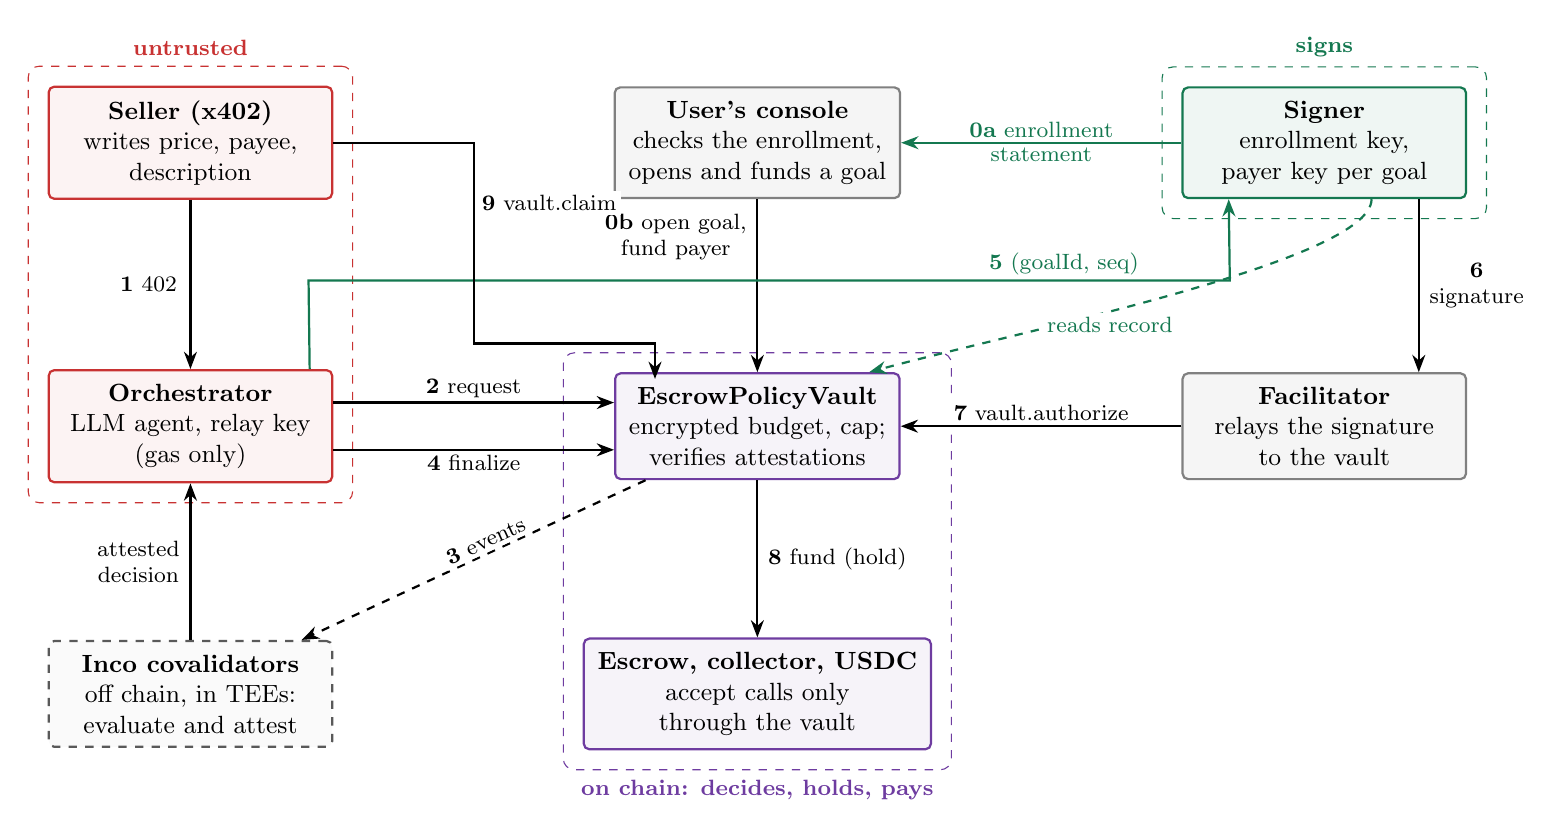
\begin{tikzpicture}[font=\small,
    pb/.style={draw,rounded corners=2pt,align=center,inner sep=5pt,minimum width=3.6cm,minimum height=1.2cm,thick},
    pl/.style={font=\footnotesize,align=center,fill=white,inner sep=1.5pt}]
  % columns at x = 0, 6.5, 13; rows at y = 0, -3.6, -7.0
  \node[pb,draw=untrusted,fill=untrusted!6] (vendor) at (0,0) {\textbf{Seller (x402)}\\writes price, payee,\\description};
  \node[pb,draw=gray,fill=gray!8] (user) at (7.2,0) {\textbf{User's console}\\checks the enrollment,\\opens and funds a goal};
  \node[pb,draw=enclave,fill=enclave!7] (signer) at (14.4,0) {\textbf{Signer}\\enrollment key,\\payer key per goal};
  \node[pb,draw=untrusted,fill=untrusted!6] (agent) at (0,-3.6) {\textbf{Orchestrator}\\LLM agent, relay key\\(gas only)};
  \node[pb,draw=chain,fill=chain!6] (vault) at (7.2,-3.6) {\textbf{EscrowPolicyVault}\\encrypted budget, cap;\\verifies attestations};
  \node[pb,draw=gray,fill=gray!8] (fac) at (14.4,-3.6) {\textbf{Facilitator}\\relays the signature\\to the vault};
  \node[pb,draw=gray!70!black,fill=gray!4,dashed] (inco) at (0,-7.0) {\textbf{Inco covalidators}\\off chain, in TEEs:\\evaluate and attest};
  \node[pb,draw=chain,fill=chain!6] (escrow) at (7.2,-7.0) {\textbf{Escrow, collector, USDC}\\accept calls only\\through the vault};

  % setup
  \draw[arr,enclave] (signer.west) -- node[pl,above]{\textbf{0a} enrollment} node[pl,below]{statement} (user.east);
  \draw[arr] (user.south) -- node[pl,pos=0.22,left=2pt]{\textbf{0b} open goal,\\fund payer} (vault.north);

  % one paid call
  \draw[arr] (vendor.south) -- node[pl,left=3pt]{\textbf{1} 402} (agent.north);
  \draw[arr] ($(agent.east)+(0,0.3)$) -- node[pl,above]{\textbf{2} request} ($(vault.west)+(0,0.3)$);
  \draw[arr] ($(agent.east)+(0,-0.3)$) -- node[pl,below]{\textbf{4} finalize} ($(vault.west)+(0,-0.3)$);
  \draw[darr] ($(vault.south west)+(0.4,0)$) -- node[pl,pos=0.45,above,sloped]{\textbf{3} events} ($(inco.north east)+(-0.4,0)$);
  \draw[arr] (inco.north) -- node[pl,left=2pt]{attested\\decision} (agent.south);
  \draw[arr,enclave] ($(agent.north east)+(-0.3,0)$) -- (1.5,-1.75) -- node[pl,pos=0.82,above]{\textbf{5} (goalId, seq)} (13.2,-1.75) -- ($(signer.south west)+(0.6,0)$);
  \draw[darr,enclave] ($(signer.south)+(0.6,0)$) .. controls (15.0,-1.5) and (10.5,-2.4) .. node[pl,pos=0.6,below]{reads record} ($(vault.north east)+(-0.4,0)$);
  \draw[arr] ($(signer.south)+(1.2,0)$) -- node[pl,right=2pt]{\textbf{6}\\signature} ($(fac.north)+(1.2,0)$);
  \draw[arr] (fac.west) -- node[pl,above]{\textbf{7} vault.authorize} (vault.east);
  \draw[arr] (vault.south) -- node[pl,right=2pt]{\textbf{8} fund (hold)} (escrow.north);
  \draw[arr] (vendor.east) -- (3.6,0) -- node[pl,pos=0.3,right=1pt]{\textbf{9} vault.claim} (3.6,-2.55) -- (5.9,-2.55) -- (5.9,-3.0);

  \begin{scope}[on background layer]
    \node[zone,draw=untrusted,fit=(vendor)(agent)] (zu) {};
    \node[zone,draw=chain,fit=(vault)(escrow)] (zc) {};
    \node[zone,draw=enclave,fit=(signer)] (ze) {};
  \end{scope}
  \node[font=\footnotesize\bfseries,text=untrusted,anchor=south] at (zu.north) {untrusted};
  \node[font=\footnotesize\bfseries,text=chain,anchor=north] at (zc.south) {on chain: decides, holds, pays};
  \node[font=\footnotesize\bfseries,text=enclave,anchor=south] at (ze.north) {signs};
\end{tikzpicture}
}
\caption{Architecture and one paid call. Red components read attacker-controlled text. Inco's covalidators
evaluate off chain and attest; the vault verifies the attestation on chain. The signer's only input from the
orchestrator is $(\mathit{goalId}, \mathit{seq})$, and its signature moves money only through the vault's
\code{authorize} (7, 8); the vendor is paid by \code{claim} through the vault (9).}
\label{fig:arch}
\end{figure*}

\subsection{Overview}

Figure~\ref{fig:arch} shows the components. The \emph{orchestrator} runs the language model and an x402
client, and is untrusted. The \code{EscrowPolicyVault} contract holds each user's policy, records every
request and decision, and is the operator of every escrowed payment. The \emph{signer} holds the enrollment
key and the payer keys. The user acts once per \emph{goal}: the console obtains an enrollment statement for a
fresh payer, checks it, sends \code{openEnrolledGoal} from the user's wallet with an encrypted budget, an
encrypted per-call cap, a public call count, a public attempt budget, an expiry and a payee allowlist, and,
once that transaction has a few confirmations, funds the payer with an amount chosen independently of the
budget (Section~\ref{sec:otherleak}). The user's wallet grants no allowance and never signs a payment.

A paid call proceeds as follows. The orchestrator receives a 402, parses it strictly, and lets the model decide
only whether to proceed; amount, payee and asset come from the parser. The relay key submits
\code{requestEscrowSpend(goalId, amount, payTo, resource, payBy, captureDeadline, keyHash)}. After Inco
evaluates the request, anyone may submit the attested decision to \code{finalizeDecision}. The orchestrator
asks the signer to authorize $(\mathit{goalId}, \mathit{seq})$ and attaches the signature to its retry. The
vendor's facilitator calls the vault's \code{authorize}, which funds the escrow, and the vendor then calls the
vault's \code{claim} to be paid. A paid call is four transactions, one of them the vendor's.
Figure~\ref{fig:seq}, after the references, gives every message.

\subsection{Authenticated enrollment}
\label{sec:enrollment}

The user funds the payer, and the payer's address reaches the console from the signer through the
orchestrator. Under A2 that path can substitute an address the attacker holds, and the user would fund it
directly: no request, policy or signature would be involved. Earlier versions of this system stated this as
a limit. Enrollment closes it.

\paragraph{Derivation.} The console draws a fresh 32-byte \emph{enrollment identifier} $e$ and asks for a
payer for its own wallet $o$. The signer derives the payer's key from the identifier
$\mathit{payer}/\mathit{chainId}/\mathit{vault}/o/e$ and returns the address with a statement
$\sigma_E$, an EIP-712 signature by its \emph{enrollment key} over $(\mathit{payer}, o, e)$, whose domain names
the chain and the vault. Because the payer is a function of $o$, no statement for a payer can ever name a
different owner: not one requested by a hostile orchestrator, and not one issued after a restart that lost the
signer's memory. The signer keeps no state about payers; the goal record names the owner and the vault records
$e$, so the key for any goal is re-derived from the chain. The enrollment key's identifier names only the
chain, so its address can be read before the vault that pins it is deployed.

\paragraph{Checks.} The vault fixes the enrollment address at deployment and accepts
\code{openEnrolledGoal}$(\mathit{params}, e, \sigma_E)$ only if $\sigma_E$ recovers to it for
$(\mathit{params.payer}, \mathit{msg.sender}, e)$; the unchecked \code{openGoal} reverts. The console, before
sending anything, checks the statement against the enrollment address built into it, compares that address
with the vault's \code{enrollmentSigner()} through its own RPC endpoint, and checks the owner, identifier, chain
and vault. Before funding it waits three blocks after the setup transaction and re-reads that the vault binds
this payer to this goal, that the goal is this wallet's, and that it was opened under $e$.

\paragraph{The connection to the measurement.} In a ROFL deployment the enrollment key is derived by Oasis's key
manager from the application's identity and the identifier \code{enrollment/<chainId>}, and released only to
instances the application's on-chain policy admits. That policy lists the accepted enclave measurements. A valid
statement therefore comes from an admitted instance, unless the key manager or the administrator who sets the policy
is compromised. On a laptop the key comes from a seed file, and a statement means only that whoever holds the file
signed it. We deployed the vault both ways and say for each run which one it used (Section~\ref{sec:liveeval}).

\paragraph{Finality of setup.} The adversary model allows dropped blocks, so a confirmed setup can disappear after
the user has funded the payer. The payer is then unbound, but every statement for it names this owner, and the vault
reads the owner from the sender, so no other wallet can bind it; the owner can open the goal again with the same
statement, and the funds wait in a payer only this owner's goal can use. Front-running fails for the same reason: a
statement seen in the mempool opens nothing for another sender. The confirmations narrow the window; they do not
carry the argument.

\subsection{Policy state and the debit}
\label{sec:writeahead}

For each goal the vault stores the remaining budget $B$ and the cap $C$ as encrypted handles, and the call count
$n$, attempt budget $m$, allowlist $A$, asset, expiry and relay in plaintext. The requested amount is public by
design: were it encrypted, the orchestrator could submit one ciphertext to the check and other terms to the signer.
Structural conditions (caller is the relay, goal open and unexpired, payee in $A$, non-zero amount, hold not passed,
an attempt left, no request pending) revert. Policy conditions (budget, cap and call count) resolve into a recorded
approval or rejection, so a refused request stays visible on chain.

The debit is written as a selection, since a contract cannot branch on an encrypted value:

\begin{lstlisting}[language=Solidity]
ok     = B[g].ge(a).and(C[g].ge(a));             // encrypted: a <= B and a <= C
debit  = ok.select(a.asEuint256(), uint256(0).asEuint256());
B[g]   = B[g].sub(debit);  B[g].allowThis();     // new handle, retained by the vault
ok.reveal();                                     // only the decision becomes public
\end{lstlisting}

All of this runs in the transaction that records the request, its sequence number $s$, a hash of its terms and a
frozen validity window. If the public call count is zero the vault records a rejection without touching the budget.
Both limits are combined in one condition, so a rejection does not say which limit refused. The call count moves at
finalization, and only on approval, which is why requests on a goal are strictly sequential.

This \emph{write-ahead} debit is a construction choice, not a security principle the bound needs. With one request
pending per goal, a design that debited at finalization, before any approval could be signed, would satisfy the same
invariants; ours is what Inco makes expressible, since the debit must be computed where the comparison is. What the
choice changes is the accounting: a pending request has already debited, so the invariants of
Section~\ref{sec:model} carry a term $Q$ for it. Selecting the operand, not the result, keeps the subtraction defined
on every path. Every debit produces a new budget handle to which only the vault is granted access.

\subsection{Finalization and the signer}
\label{sec:signer}

\code{finalizeDecision}$(g, s, v, \sigma)$ verifies that the covalidator signatures $\sigma$ attest plaintext $v$ for
\emph{the decision handle stored for $(g, s)$}, never one the caller supplies. Anyone may call it.

The signer accepts $(g, s)$ and nothing else. It reads the goal and the request, refuses unless the request is finalized,
approved, not reclaimed, on an open goal, in the expected asset and inside its frozen window, re-derives the payer's key
from the goal's owner and enrollment identifier, and refuses if that key is not the goal's payer. It then signs one kind of
message: a \code{receiveWithAuthorization} from the payer to the pinned collector, described in Section~\ref{sec:binding}.
The operator, collector, escrow and token come from configuration fixed at boot, never from the chain, and the signer has no
code path to a plain transfer. The record is frozen, so repeating the query gives a byte-identical signature. These refusals
tell a caller why nothing was signed; since the vault checks again when money moves, they are not what makes a signature safe.

After the owner closes a goal, the signer also signs a \emph{sweep} of the payer's remaining balance, payable to the goal's
owner, through the vault's \code{charge}, which checks on chain that the goal is closed, the receiver is its owner and no fee is
taken.

\subsection{Collection through the escrow}
\label{sec:escrow}

An EIP-3009 transfer signed for an approved request stays valid whatever later happens to the approval. In version~1 of this work
that put the signer's RPC inside the trusted base: an invented approval reported by a malicious endpoint would be signed, and a
signature released for an approval on a dropped branch survived the branch. With $B_0 = C = 0.20$ and $n_0 = 1$, an approval of
0.10 on a discarded branch and a canonical approval of 0.20 at the same sequence number carried different nonces, so the token
accepted both and paid 0.30. Waiting for finality was not practical: on 6 November 2026 Base Sepolia's \code{safe} block was about
23 minutes behind the head and its \code{finalized} block 3.8 hours, against a 60-second hold.

In the escrow design the vault is the operator of every payment. The vault's \code{authorize} derives the payment from its own record
and requires the caller's struct to equal it in every field, the record to be finalized, approved and not reclaimed, the goal to be open,
the amount to be the whole recorded amount, and the collector to be the pinned one; only then does it call the escrow. In the example
above, the 0.10 signature names a record that does not exist on the canonical chain, so it is refused and the payment is 0.20. The
inherited \code{requestSpend} reverts on this vault, so a goal has no other way to spend.

\begin{table*}[t]
\centering\small
\begin{tabular}{@{}L{0.3\linewidth}L{0.2\linewidth}L{0.44\linewidth}@{}}
\toprule
Escrow state & Time & \code{reclaimExpired} \\
\midrule
Not funded & before \textit{validBefore} & refused: the signature is still live \\
Not funded & from \textit{validBefore} & credit: token and escrow both refuse the signature from then on \\
Held & before capture deadline & refused: the vendor can still claim \\
Held & from capture deadline & void, funds to payer, credit \\
Funded, nothing held, nothing captured & any & credit: the payer took the funds back directly \\
Captured & any & refused: paid \\
\bottomrule
\end{tabular}
\caption{What decides a reclaim. The state is read from the escrow.}
\label{tab:reclaim}
\end{table*}

An approved request has three endings: paid, returned, or never funded. Table~\ref{tab:reclaim} gives the rule for crediting it back.
The vendor captures with \code{claim}$(g, s, k)$, which only the recorded payee may call and which requires a preimage of the request's
key hash if one was set. Closing a goal stops funding, because \code{authorize} requires an open goal; funds already held can be claimed
until their deadline and come back through a reclaim after it.

\subsection{The end-to-end binding}
\label{sec:binding}

Several contracts stand between a signature and a payment, and the loss bound depends on all of them. We state what binds what, for the
deployments our runs used.

\paragraph{The signed message.} The payer signs, under USDC's EIP-712 domain (name, version, chain id, token address),
$\code{ReceiveWithAuthorization}(\mathit{from} = \mathit{payer}, \mathit{to} = \mathit{collector}, \mathit{value} = \mathit{maxAmount},
\mathit{validAfter} = 0, \mathit{validBefore} = \mathit{preApprovalExpiry}, \mathit{nonce})$, where
\begin{align*}
h_0 &= \mathrm{keccak}(\mathrm{enc}(\mathit{TYPEHASH}, \mathit{info}[\mathit{payer} := 0])),\\
\mathit{nonce} &= \mathrm{keccak}(\mathrm{enc}(\mathit{chainId}, \mathit{escrow}, h_0))
\end{align*}
is the escrow's own payment hash with the payer zeroed, and $\mathrm{enc}$ is ABI encoding. The nonce therefore covers every field of
\code{PaymentInfo} except the payer (operator, receiver, token, maximum amount, the three deadlines, fee bounds, fee receiver and salt),
plus the chain and the escrow; the payer is covered by \textit{from}. The salt is $(g \ll 64) \mathbin{|} s$, which makes the nonce
unique per request and lets the vault find the record.

\paragraph{Who may submit it.} USDC accepts \code{receiveWithAuthorization} only from \textit{to}, the collector. The collector acts only
when called by the escrow, and checks that the nonce equals the escrow's payer-agnostic hash of the payment it is given. The escrow accepts
\code{authorize} and \code{charge} only from the payment's operator, the vault. So a signature can move tokens only inside the vault's
\code{authorize} or \code{charge}, and both re-derive the payment from the vault's record.

\paragraph{Every other route.} The escrow's operator-only functions are \code{authorize}, \code{charge}, \code{capture}, \code{void} and
\code{refund}. The vault calls \code{authorize} after its checks, \code{charge} only for a sweep to the owner of a closed goal, \code{capture}
only in \code{claim} for the recorded payee and the whole amount with no fee, and \code{void} only in a reclaim after the capture deadline. It
never calls \code{refund}. The payer's own \code{reclaim} returns a hold to the payer after the capture deadline, which Table~\ref{tab:reclaim}
counts. Because the vault never refunds and captures only the whole amount, the escrow's \code{refundableAmount} is non-zero exactly when a
payment was captured, which is what lets \code{reclaimExpired} tell ``paid'' from ``returned''. In another integration that called
\code{refund}, that inference would fail.

\paragraph{Versions and code identities.} The escrow is commerce-payments v1.1.0~\cite{commercepayments} (commit \code{6b0a5ef}), at
\code{0xf968\ldots{}B19c} on Base and Base Sepolia, with the ERC-3009 collector at \code{0x8612\ldots{}ab88}. Neither is a proxy. At Base Sepolia
block 56{,}480{,}000 the keccak hashes of their deployed code begin \code{0x33558f6c} and \code{0xe27322c8}, and the escrow's token-store
template's \code{0x8ff35d5d}. USDC is Circle's upgradeable proxy (code hash \code{0xedc5281a}), with implementation \code{0xd74c\ldots{}C5B5}
(\code{0x1254951e}) at that block; an upgrade by its administrator is outside our model. The repository's test fixture records the code and
every storage slot these contracts read, at that block.

\subsection{The recorded funding deadline}
\label{sec:hold}

x402 offers no reservation. We take the vendor's deadline $T$ to be the end of the payment window it declares: the orchestrator records when the
402 arrived, adds \code{maxTimeoutSeconds} and passes the result as \textit{payBy}. The vault sets
\[
  \mathit{validBefore} = \min(\mathit{payBy},\ t_{\mathrm{request}} + 1\,\mathrm{h},\ \mathit{expiry}),
\]
after which the token and the escrow both refuse to fund the payment, and records a capture deadline at or after \textit{validBefore}, at most one
hour later and not past the goal's expiry, after which the escrow refuses capture. What the implementation guarantees is therefore a
\emph{recorded funding deadline}: funding before \textit{validBefore}, capture before the capture deadline. It does not guarantee that
\textit{payBy} equals the vendor's own deadline (under A2 the orchestrator chooses it, within the hour), that capture happens before $T$, that the
vendor still holds what it offered, or that funding causes delivery. Even an honest orchestrator computes \textit{payBy} from a relative timeout, so
transit delay and a difference between the vendor's clock and the chain's need a margin.

Before committing, the orchestrator checks that enough of the hold remains for the request to be funded. The threshold is a heuristic, set from
measurement: in our runs the time from the request to funding had a maximum of \fundingmax\,s (Section~\ref{sec:eval}), and the check uses
\fundingcheck\,s. It is not a guarantee of success.

Approval does not move money. A crash, an abandoned request or a vendor that never claims can leave the budget reduced by money that was not paid.
\code{reclaimExpired}$(g, s)$ returns the amount to the budget and the call to the count in the cases of Table~\ref{tab:reclaim}. Anyone may call it, since
every condition is read from the chain. It needs finalization first, so a request whose decision Inco never reveals cannot be reclaimed; the owner's
close and sweep is then a separate recovery. Reclaim restores accounting and not necessarily the ability to spend: the goal must still be open, unexpired
and have an attempt left.

\subsection{The attempt budget}
\label{sec:attempts}

Every requested amount and every decision is public, so each request answers one question about the encrypted limits: is $a \le \min(B, C)$?
Whoever chooses the amounts chooses the questions. Rejections never consumed anything, and once reclaim existed an approval left to expire consumed
nothing either: name a \textit{payBy} one second away, never fund, reclaim. Our regression test recovers a secret cap of 137{,}391 units exactly in 23
requests by binary search, reclaiming every approval, so budget and call count end where they began. This is the general lesson of the paper's second
contribution: a mechanism that restores spending capacity also restores the ability to ask, and in a private policy asking is what leaks.

The goal therefore carries a public attempt budget $m \ge n_0$, set by the owner. Every request spends one attempt, approved or rejected, and nothing
returns it. The attempt is kept apart from the call: a call is a payment the owner agreed to fund and comes back if unused, an attempt is a question
already answered. The attempt budget is also a resource a vendor can exhaust: quotes above the limits make an honest agent spend attempts on
rejections. Section~\ref{sec:leakeval} measures the trade between leakage and honest completion.

\subsection{Execution traces}

Each run produces a hash-chained trace whose payment steps carry the decision handle, the covalidator signatures and the commit transaction;
rejected attempts stay in it. Only a Merkle root is stored on chain, once per (vault, goal). The anchor is permissionless and its first write is final,
so anyone can occupy a goal's slot with an arbitrary root; verification rejects that root, at a cost in audit availability only.


\begin{figure*}[t]
\centering
\resizebox{\linewidth}{!}{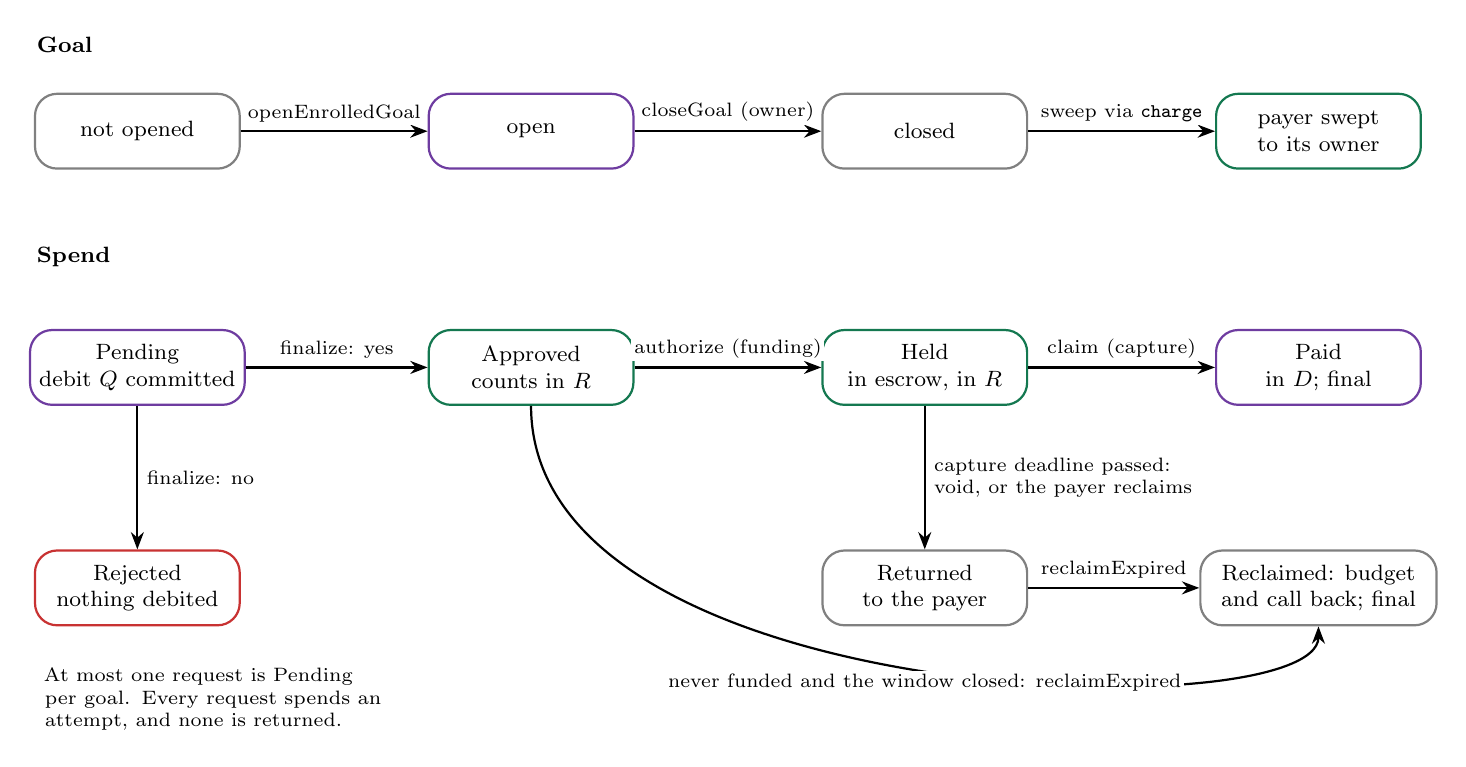
\begin{tikzpicture}[st/.style={draw,rounded corners=8pt,thick,font=\footnotesize,align=center,minimum height=0.95cm,minimum width=2.6cm,fill=white}]
  \node[font=\footnotesize\bfseries,anchor=west] at (-1.4,1.1) {Goal};
  \node[st,draw=gray] (none) at (0,0) {not opened};
  \node[st,draw=chain] (open) at (5.0,0) {open};
  \node[st,draw=gray] (closed) at (10.0,0) {closed};
  \node[st,draw=enclave] (swept) at (15.0,0) {payer swept\\to its owner};
  \draw[arr] (none) -- node[lbl,above=2pt]{openEnrolledGoal} (open);
  \draw[arr] (open) -- node[lbl,above=2pt]{closeGoal (owner)} (closed);
  \draw[arr] (closed) -- node[lbl,above=2pt]{sweep via \code{charge}} (swept);

  \node[font=\footnotesize\bfseries,anchor=west] at (-1.4,-1.6) {Spend};
  \node[st,draw=chain] (pend) at (0,-3.0) {Pending\\debit $Q$ committed};
  \node[st,draw=untrusted] (rej) at (0,-5.8) {Rejected\\nothing debited};
  \node[st,draw=enclave] (app) at (5.0,-3.0) {Approved\\counts in $R$};
  \node[st,draw=enclave] (held) at (10.0,-3.0) {Held\\in escrow, in $R$};
  \node[st,draw=chain] (paid) at (15.0,-3.0) {Paid\\in $D$; final};
  \node[st,draw=gray] (ret) at (10.0,-5.8) {Returned\\to the payer};
  \node[st,draw=gray,minimum width=3.0cm] (rec) at (15.0,-5.8) {Reclaimed: budget\\and call back; final};
  \draw[arr] (pend) -- node[lbl,above=2pt]{finalize: yes} (app);
  \draw[arr] (pend) -- node[lbl,right=2pt]{finalize: no} (rej);
  \draw[arr] (app) -- node[lbl,above=2pt]{authorize (funding)} (held);
  \draw[arr] (held) -- node[lbl,above=2pt]{claim (capture)} (paid);
  \draw[arr] (held) -- node[lbl,right=2pt,align=left]{capture deadline passed:\\void, or the payer reclaims} (ret);
  \draw[arr] (ret) -- node[lbl,above=2pt]{reclaimExpired} (rec);
  \draw[arr] (app.south) .. controls (5.0,-7.4) and (15.0,-7.6) .. node[lbl,below,pos=0.5]{never funded and the window closed: reclaimExpired} (rec.south);
  \node[font=\scriptsize,align=left,text width=4.4cm,anchor=north west] at (-1.3,-6.7) {At most one request is Pending per goal. Every request spends an attempt, and none is returned.};
\end{tikzpicture}
}
\caption{Lifecycle of a goal and of one request, with the accounting term each state counts in (Section~\ref{sec:model}).}
\label{fig:states}
\end{figure*}

\section{Security Analysis}
\label{sec:security}

Property~\ref{prop:text} and Theorem~\ref{prop:loss} hold under A2, for a goal whose enrollment was authentic and whose signer is
uncompromised, with Inco satisfying I1 to I4. Property~\ref{prop:hold} is about the recorded deadline. Theorem~\ref{prop:leakproof} is about
the decision channel and states its own assumptions. The arguments are by hand over the transition model below; we have not mechanised them.
Section~\ref{sec:eval} reports how each is tested and with what.

\subsection{Transition model}
\label{sec:model}

Fix a goal opened with budget $B_0$, cap $C$, call count $n_0$, attempt budget $m_0$, allowlist $A$ and funding $F$. Each request $s$ is in
one state: \textsf{Pending}, \textsf{Rejected}, \textsf{Approved} (finalized, not funded), \textsf{Held} (funded, not captured),
\textsf{Paid}, or \textsf{Reclaimed}. A held payment the payer took back, or one past its deadline not yet voided, is still \textsf{Held} in
the vault's accounting until it is reclaimed (Figure~\ref{fig:states}). Write $a_s$ for its amount and define
\begin{itemize}
  \item $D = \sum_{s \in \textsf{Paid}} a_s$, the lifetime vendor payments;
  \item $R = \sum_{s \in \textsf{Approved} \cup \textsf{Held}} a_s$, the reserved, unresolved amounts;
  \item $Q = a_p \cdot [\,\mathit{ok}_p\,]$, the debit of the pending request $p$, if there is one;
  \item $L = |\textsf{Approved} \cup \textsf{Held} \cup \textsf{Paid}|$, the live approvals,
\end{itemize}
where $\mathit{ok}_p$ is the pending request's encrypted decision, which exists from the request on and is revealed later. Let $B$ be the
plaintext of the budget handle, $n$ the call count, $m$ the attempts left and $\sigma$ the last sequence number. The claims are
\begin{itemize}
  \item[(J1)] $B + D + R + Q = B_0$;
  \item[(J2)] $n + L = n_0$;
  \item[(J3)] $m + \sigma = m_0$;
  \item[(J4)] no request is both \textsf{Paid} and \textsf{Reclaimed}, and each is reclaimed at most once.
\end{itemize}
J2 counts \textsf{Paid} approvals and leaves the pending request out, because the call count moves at finalization.

\begin{table*}[t]
\centering\small
\begin{tabular}{@{}L{0.17\linewidth}L{0.31\linewidth}L{0.46\linewidth}@{}}
\toprule
Transition & Effect & Why J1 to J4 are preserved \\
\midrule
request $(a)$ & $\sigma{+}1$, $m{-}1$; $B \mathrel{-}= a\cdot\mathit{ok}$; new \textsf{Pending} & $Q$ rises by exactly what $B$ falls (J1); $m + \sigma$ fixed (J3). Only with no request pending, so $Q$ was 0. If $n = 0$, $\mathit{ok} = 0$ in plaintext. \\
finalize, approved & \textsf{Pending}$\to$\textsf{Approved}; $n{-}1$ & $Q$ moves into $R$ (J1); $L{+}1$, $n{-}1$ (J2). Needs $n \ge 1$, guaranteed since $\mathit{ok}$ required it at request (I1, I2). \\
finalize, rejected & \textsf{Pending}$\to$\textsf{Rejected} & $Q = 0$ before and after (J1). \\
authorize (fund) & \textsf{Approved}$\to$\textsf{Held} & Stays in $R$ and $L$. Refused unless approved, not reclaimed, goal open, terms and amount exact. \\
claim (capture) & \textsf{Held}$\to$\textsf{Paid} & $a$ moves from $R$ to $D$ (J1); stays in $L$ (J2). Escrow refuses after the capture deadline. \\
payer's reclaim & funds back to payer & No accounting change: still \textsf{Held} in the vault until credited. \\
reclaimExpired & \textsf{Approved}/\textsf{Held}$\to$\textsf{Reclaimed}; $B{+}a$, $n{+}1$ & $a$ moves from $R$ to $B$ (J1); $L{-}1$, $n{+}1$ (J2); $m$ unchanged (J3). Only in Table~\ref{tab:reclaim}'s cases, never from \textsf{Paid}; a flag stops a second credit (J4). \\
close, sweep & goal closed; payer's balance to owner & No accounting change; \code{authorize} and \code{requestEscrowSpend} then refuse. \\
\bottomrule
\end{tabular}
\caption{Every transition of a goal and why it preserves the invariants. A reclaim of an older approval while a newer request is
pending changes $R$ and $B$ only, and leaves $Q$ as it was.}
\label{tab:transitions}
\end{table*}

\begin{proposition}[Invariants]\label{prop:inv}
Under I1 to I4, J1 to J4 hold in every reachable state of a goal on the canonical chain.
\end{proposition}

\noindent\emph{Proof.} Initially $B = B_0$, $n = n_0$, $m = m_0$, $\sigma = 0$ and all sums are zero. Table~\ref{tab:transitions} lists
every function that changes a goal's state and shows each preserves J1 to J4; anything else reverts or leaves the goal unchanged.
Two points need the assumptions. J1 equates a plaintext with handle arithmetic, which needs I1 and I2: the budget handle each request reads
is the one the previous transaction wrote. And the \textsf{Approved}/\textsf{Rejected} split equals $\mathit{ok}$ only if the finalized value
is the attested one, which is I3 together with the vault verifying against the handle it stored. \hfill$\square$

\begin{property}[No authority from text]\label{prop:text}
No signature issued by the signer moves money to anyone other than the goal's owner unless the vault's record on the canonical chain holds
$(g, s)$ as finalized, approved and not reclaimed when the payment is funded, and the signed terms equal the terms recorded at request time.
\end{property}

\noindent The signer consumes no terms from its caller, and by Section~\ref{sec:binding} a signature moves tokens only inside the vault's
\code{authorize}, which re-derives and compares the whole payment, or \code{charge}, which pays only the owner of a closed goal.

\begin{theorem}[Lifetime loss bound]\label{prop:loss}
Under A2, for a goal whose enrollment was authentic and whose signer is uncompromised, with Inco satisfying I1 to I4, the lifetime vendor
payments satisfy $D \le \min(B_0, C\cdot n_0)$, every payment goes to a member of $A$, and each is at most $C$. Separately, vendor payments and
sweeps together never exceed the payer's funding $F$ plus any tokens others sent it: held funds that return to the payer are counted once, when
they are paid or swept. The bound holds whatever the signer's RPC reports and whatever blocks are dropped after the enrollment is stable.
Gas, the relay key's spending and lost availability are outside it.
\end{theorem}

\noindent\emph{Proof.} By J1, $D \le B_0$, since $B$, $R$ and $Q$ are non-negative. Every paid request was approved, and approval needs
$a \le C$ by I1 and I3, so each payment is at most $C$. Paid requests are live approvals, so $|\textsf{Paid}| \le L \le n_0$ by J2, and
$D \le C\cdot n_0$. Payees are checked against $A$ structurally at request, and capture pays the recorded payee. By Property~\ref{prop:text}
only records on the canonical chain count, which is why neither the RPC nor a dropped block can add to $D$. For the second bound, every
token that leaves the payer goes to the escrow or to the owner; the escrow pays out only by capture or returns to the payer, so the payer's
balance plus held funds plus $D$ plus sweeps equals $F$ plus inflows at all times. Authentic enrollment is needed because otherwise the payer
the user funds might not be the one the goal names; an uncompromised signer because the payer is a key. \hfill$\square$

\begin{property}[Recorded funding deadline]\label{prop:hold}
A signature for a request cannot fund the escrow at or after its recorded \textit{validBefore}, and the vendor cannot capture at or after the
recorded capture deadline. Whatever the orchestrator reports, no payment is funded an hour or more after its request, or captured two hours or
more after it.
\end{property}

\noindent The window is frozen in the record and is the one signed; the token and the escrow enforce it. This is a property of the recorded
deadline only. It protects a buyer against a late-collecting vendor if the orchestrator reports the hold honestly and with a margin for transit and
clocks; under A2 it weakens to the hour, without weakening Theorem~\ref{prop:loss}. Authenticated commercial holds need the vendor's signature on
an absolute deadline, as in Section~\ref{sec:delivery}.

\begin{property}[Reclaim cannot double-pay]\label{prop:reclaim}
For every $(g, s)$, the amount is never both captured and credited back, and is credited at most once.
\end{property}

\noindent This is J4. A credit needs nothing captured. If nothing was funded, it needs $t \ge \mathit{validBefore}$, after which funding is
impossible. If funds are held, it needs the capture deadline to have passed, after which capture is impossible, and the funds are voided in the
same transaction.

\subsection{The decision channel}
\label{sec:leakthm}

\begin{definition}[Decision-channel leakage]\label{def:leak}
The secret is $\mathsf{s} = (B_0, C)$ and $P$ is the public setup: everything public before the first request, including the funded amount,
expiry and allowlist. The pair $(\mathsf{s}, P)$ has any joint distribution, and every goal has attempt budget at most $m$. Before request $i$ an
adaptive adversary chooses which earlier approvals $\rho_i$ to reclaim and an amount $a_i$, as functions of $P$, its coins $r$ and everything
public so far, and observes $d_i = [\,n_i \ge 1\,] \wedge [\,a_i \le B_i\,] \wedge [\,a_i \le C\,]$. Its view after $k \le m$ requests is
$V = (\rho_1, a_1, d_1, \ldots, \rho_k, a_k, d_k)$. The leakage is $\mathcal{L} = H_\infty(\mathsf{s} \mid P) - H_\infty(\mathsf{s} \mid P, V)$, with
$H_\infty(X \mid Y) = -\log_2 \sum_y \max_x \Pr[x, y]$ the average conditional min-entropy~\cite{smith2009}.
\end{definition}

\begin{theorem}[Decision-channel bound]\label{prop:leakproof}
Assume that the adversary's coins are independent of $\mathsf{s}$ given $P$, and that no decision is revealed for a request that does not end on
the canonical chain. Then for every prior and every adversary strategy, $\mathcal{L} \le m$ bits.
\end{theorem}

\noindent\emph{Proof.} For each fixed $(p, r)$ each $a_i$, $\rho_i$ and the decision to stop are functions of $d_1, \ldots, d_{i-1}$, so the view is
determined by the decision bits. These form the leaves of a binary tree of depth at most $m$, so the view takes at most $2^m$ values $v$. Hence
$\sum_v \max_{\mathsf{s}} \Pr[\mathsf{s}, v \mid p, r] \le 2^m \max_{\mathsf{s}} \Pr[\mathsf{s} \mid p]$. Multiplying by $\Pr[p, r]$ and summing gives
$H_\infty(\mathsf{s} \mid P, V, r) \ge H_\infty(\mathsf{s} \mid P) - m$, the bound for deterministic channels of Smith~\cite{smith2009}. The second
assumption is what makes the depth $m$: an attempt is counted on the canonical chain, so a decision revealed for a request on a branch that is later
dropped would be an answer the count never charged. \hfill$\square$

\paragraph{From the channel to the deployed transcript.} The theorem bounds what the decisions reveal. Relating it to everything the deployed
system publishes needs further assumptions, which we state and do not prove. (i) Ciphertexts, handles, Inco's operation events and attestations
reveal nothing about $\mathsf{s}$ beyond the decisions; this is I5 together with handles being computed from operation inputs and not from
plaintexts, which is how Lightning derives them, and needs a computational argument we have not made. (ii) There are no timing or gas channels.
In one measurement on version~1's design both outcomes used 326{,}528 gas, and over 50 calls decision latency showed overlapping distributions,
which does not rule a channel out. (iii) No revealed decision is on a dropped branch; we have not measured how soon Inco reveals relative to
finality on Base. (iv) The user, client and console reveal nothing derived from the limits; Section~\ref{sec:otherleak} gives two ways an earlier
console did. (v) Each goal has its own secret; a user who reuses limits across goals gives an adversary up to the sum of their attempt budgets.

\paragraph{The bound is an average and a ceiling.} With a cap uniform on $0, \ldots, 1023$, a request for one unit that is rejected identifies
$C = 0$ from a single decision. And the bound can be close to tight: binary search narrows the cap's range by a factor of two per answer. Our
regression test, with a 10 USDC range, leaves an interval of 0.117 to 0.156 USDC after $m = 8$ and recovers the cap at $m = 30$.
Section~\ref{sec:leakeval} asks what the bound leaves in practice.

\subsection{What the bound does not cover}
\label{sec:otherleak}

\paragraph{Spending.} The vault never sees the 402 body, so a compromised orchestrator may request more than the seller asked, up to the cap, to an
allowlisted payee. A vendor that is paid and delivers nothing is paid. An allowlisted vendor that signs an inflated price is paid that price within
the limits. Removing the first needs a vendor-signed quote the vault verifies; the others are Section~\ref{sec:delivery}'s subject.

\paragraph{Leakage outside the decisions.} The payer's token balance is public, so funding it with the budget plus a margin, as an earlier console
did, publishes the budget before any request. The console now funds a fixed 5.00 USDC, above the largest budget it accepts, at the cost of a looser
fallback bound. An earlier console also priced its overcharge test vendor from the budget and passed that through the orchestrator. Every value a
deployment sends must be checked; the console's own defaults are constants in public code and so are not secrets.

\paragraph{Liveness.} A decision Inco never reveals blocks the goal, since only finalization clears a pending request; no money is at risk and the
owner can close the goal and sweep. On Base Sepolia, reveals need both of two covalidators, and the orchestrator refuses to commit a debit unless Inco
can reveal a known handle. A lying RPC can stall a run or waste a signature.

\section{Key-Release Delivery for Digital Goods (Specified)}
\label{sec:delivery}

Theorem~\ref{prop:loss} stops at capture: a vendor that captures and delivers nothing is paid, within the limits. This section specifies one
protocol that extends the protection to delivery, for one kind of good, with both parties' protection and the assumptions it needs. The
dispute predicate is built and measured; the vault's order states, the bond and the window are not built, and Section~\ref{sec:eval} does not
evaluate them.

\paragraph{Scope.} A \emph{digital good} here is a byte string $M$ of at most 4 KiB whose hash $h_m = H(M)$ the vendor commits to before payment.
That covers a quote, a model's answer or a record computed before the 402 is sent; larger goods need a chunked commitment, which we leave to future work.
The protocol decides whether the vendor released a key that opens a committed ciphertext to the committed bytes. It does not decide whether those bytes
are what the buyer wanted; a named data source that signs $h_m$ is the protocol's only way to give them meaning, and quality no such signature captures is
out of scope.

\subsection{The protocol}

\paragraph{Offer.} The vendor draws a fresh key $k$, encrypts $M$ with a keccak keystream (block $i$ of the ciphertext is block $i$ of $M$ XOR
$\mathrm{keccak}(k, i)$, 32-byte blocks), and answers the buyer's request with $c$ and an EIP-712 offer $\sigma_V$ over (resource, asset, payee, price,
$h = H(k)$, $h_c = H(c)$, $h_m$, a fresh order identifier, the buyer named in the request, the vault, the last acceptance time $T_a$ and the delivery
deadline $T$), signed by the key the vendor registered with its bond. Fresh $k$ per order is required: the keystream is not secure under key reuse.

\paragraph{Acceptance.} The buyer's client checks $H(c) = h_c$ and keeps $c$; a buyer that does not hold $c$ must not accept. The relay submits the request
with $\sigma_V$. The vault verifies the signature against the vendor's registered key, that the order identifier is unused and names this buyer, that the
price is the signed price, and that $t < T_a$, with $T - T_a$ at least the agreed inclusion delay $\delta$. The request then goes through the same encrypted
check and debit as any other. On approval the payment is funded into the escrow and locked against $(h, h_c, h_m, T)$, and the vendor's penalty $\pi$ is
reserved from the free balance of its bond in the same transaction, which reverts if too little is free. An order exists only once funded and locked.
Acceptance means this atomic funded transition, not submission of the request: funding rechecks the signature, unused order identifier and
$t < T_a$. Approval that arrives too late creates no order and no penalty liability; its unused reservation can be reclaimed under the base policy.
The order identifier becomes used only at funding. Thus confidential evaluation cannot shorten the vendor's promised response margin.

\paragraph{Release and capture.} The vendor calls \code{claim}$(k)$ before $T$. The vault checks $H(k) = h$, records $k$, and starts a dispute window $W$;
publishing $k$ enables decryption. After $W$ without a valid dispute the escrow captures to the vendor and the penalty reservation is released. No valid
$k$ by $T$: anyone may void the hold, the amount returns to the budget as in a reclaim, and the penalty moves from the bond to the buyer. The trigger is
the absence of $k$ on chain, never the buyer's claim. This needs an extended escrow, not the deployed auth-capture escrow unchanged: a funded order has
exactly one terminal outcome (capture, no-key refund or successful-dispute refund), and neither payer reclaim nor goal closure can bypass its window.
The capture deadline must extend beyond $T + W + \delta$, and a timely release must remain claimable through that window. A refund atomically returns
tokens to the payer, credits the encrypted budget and restores one call exactly once; capture does neither. Neither outcome restores an attempt.
An order still awaiting its window stays reserved in $R$ and $L$ of Section~\ref{sec:model}. These are requirements for the unbuilt integration.

\paragraph{Dispute.} Within $W$, anyone holding $c$ may submit it with a dispute fee $f$. The vault checks $H(c) = h_c$ and $H(k) = h$, decrypts, and
compares $H(\mathrm{Dec}_k(c))$ with $h_m$. A mismatch voids the hold, returns the amount to the payer and the budget, pays the penalty and returns $f$; a
match pays $f$ to the vendor. A ciphertext whose hash does not match $h_c$ is invalid evidence and cannot refund the order. Our implementation of this predicate (\code{KeyReleaseVerifier}) uses 86{,}894 gas of execution for a 4{,}096-byte
ciphertext, plus about 65{,}000 for the calldata. The predicate and calldata therefore fit under 200{,}000 gas; this excludes the unbuilt order,
bond and refund logic. The fee $f$ must cover the complete dispute's gas cost at an agreed gas price, which has not yet been measured.

\subsection{What each party is protected from}

\paragraph{Buyer.} (D1) The vendor is captured to only if it published, before $T$, a $k$ with $H(k) = h$, and no valid dispute followed within $W$.
(D2) Whenever $k$ is published, a buyer that accepted holds $c$ with $H(c) = h_c$, because it checked before accepting, and can decrypt.
(D3) A vendor that does not publish $k$ by $T$, on an order accepted by $T_a$, loses $\pi$ to the buyer, decided by the chain alone.
(D4) If $\mathrm{Dec}_k(c)$ is not the committed $M$, a dispute within $W$ refunds the price and pays $\pi$. D1 follows from the hash lock and the
window, D2 from the acceptance check, D3 from the atomic reservation and the on-chain trigger, D4 from the commitments and the price held through $W$.

\paragraph{Vendor.} (V1) Once an order is locked the buyer cannot withdraw before $T$: the funds are in the escrow under the vault's control, and nothing the
buyer or its agent can do changes the order's state. (V2) A vendor whose \code{claim} is included before $T$ is captured to unless a dispute proves the
predicate false. A false dispute fails the vault's own recomputation and pays the vendor $f$. (V3) A buyer cannot lock an order so late that the vendor
has no time to claim, because acceptance ends at $T_a \le T - \delta$.

\paragraph{Key disclosure without settlement.} A \code{claim} discloses $k$ when it is broadcast, before it settles. It could then revert, be
delayed past $T$, or be included in a block that is later dropped, leaving a buyer with the good and the vendor unpaid. A claim can revert only if it is late or the key is
wrong, since after acceptance no other party can change the order (V1). A dropped block restores the order to locked with $k$ already public; the vendor
resubmits the same claim, which is valid until $T$ on the canonical chain. The vendor is therefore exposed only if its claim, submitted by $T - \delta$, is
not included by $T$ on the canonical chain, which is the same inclusion assumption D3 makes in the buyer's favour. A vendor wanting to avoid public
disclosure before inclusion can submit through a private transaction channel; we do not rely on one.

\subsection{Assumptions and what remains open}

\emph{Inclusion:} a transaction submitted $\delta$ before a deadline is included before it, on the canonical chain. \emph{An honest disputer:} under A2
the buyer's agent may decline to dispute. D4 then needs another party holding $c$, such as the user's console or a watcher the user runs; without one,
the loss is still bounded by Theorem~\ref{prop:loss}, and D1 to D3 do not depend on disputes. \emph{Privacy:} $k$ is public, so $M$ stays private only as
long as $c$ does. A dispute publishes $c$ and therefore $M$; a buyer who disputes gives up the good's confidentiality. \emph{Collusion:} the allowlist,
not the offer signature, limits which vendors can be paid; a signed offer stops an orchestrator altering an honest quote and does nothing against an
allowlisted vendor that signs an inflated one. \emph{Adoption:} a vendor must accept the vault as the escrow's operator and register a bond.

The intended bilateral protection is conditional on the extended escrow and accounting rules above, the inclusion assumption and, for D4, someone
disputing. Only the predicate has been implemented; no end-to-end fair-exchange guarantee has been established. The protocol cannot judge goods
whose value is not fixed by a commitment made before payment.
Held services, such as a reserved GPU slot, need a signed hold and a different proof of delivery, and remain future work (Section~\ref{sec:limits}).

\begin{figure*}[t]
\centering
\resizebox{0.88\linewidth}{!}{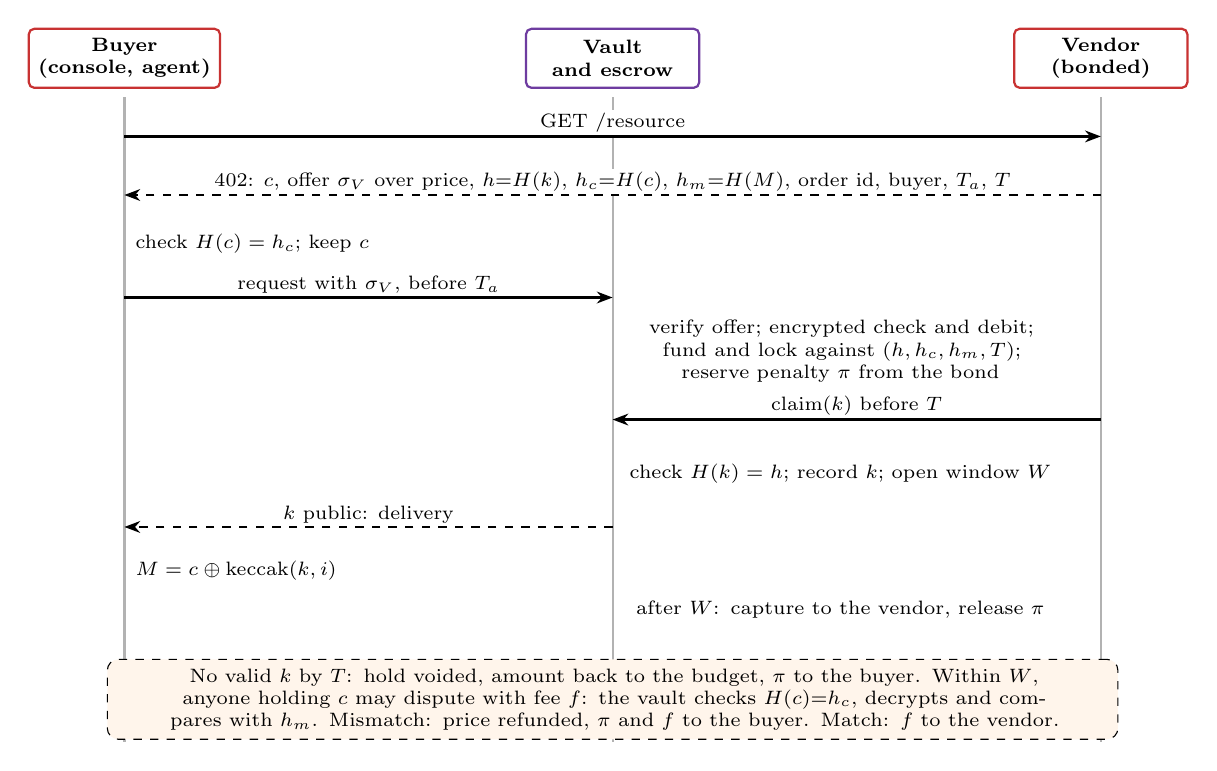
\begin{tikzpicture}[x=1cm,y=-0.62cm,
    msg/.style={-{Stealth[length=2mm]},thick},
    rmsg/.style={-{Stealth[length=2mm]},thick,dashed},
    mlab/.style={font=\scriptsize,fill=white,inner sep=1pt,align=center},
    act/.style={draw,thick,fill=white,font=\scriptsize\bfseries,align=center,minimum width=2.2cm,minimum height=0.75cm,rounded corners=2pt}]
  \def\xB{0}\def\xE{6.2}\def\xV{12.4}
  \node[act,draw=untrusted] at (\xB,0) {Buyer\\(console, agent)};
  \node[act,draw=chain]     at (\xE,0) {Vault\\and escrow};
  \node[act,draw=untrusted] at (\xV,0) {Vendor\\(bonded)};
  \foreach \x in {\xB,\xE,\xV} \draw[gray!60,thick] (\x,0.8) -- (\x,14.0);
  \draw[msg]  (\xB,1.6) -- node[mlab,above]{GET /resource} (\xV,1.6);
  \draw[rmsg] (\xV,2.8) -- node[mlab,above]{402: $c$, offer $\sigma_V$ over price, $h{=}H(k)$, $h_c{=}H(c)$, $h_m{=}H(M)$, order id, buyer, $T_a$, $T$} (\xB,2.8);
  \node[mlab,anchor=west] at (\xB+0.1,3.8) {check $H(c) = h_c$; keep $c$};
  \draw[msg]  (\xB,4.9) -- node[mlab,above]{request with $\sigma_V$, before $T_a$} (\xE,4.9);
  \node[mlab,anchor=west,text width=5.4cm] at (\xE+0.15,6.0) {verify offer; encrypted check and debit; fund and lock against $(h, h_c, h_m, T)$; reserve penalty $\pi$ from the bond};
  \draw[msg]  (\xV,7.4) -- node[mlab,above]{claim($k$) before $T$} (\xE,7.4);
  \node[mlab,anchor=west,text width=5.4cm] at (\xE+0.15,8.5) {check $H(k) = h$; record $k$; open window $W$};
  \draw[rmsg] (\xE,9.6) -- node[mlab,above]{$k$ public: delivery} (\xB,9.6);
  \node[mlab,anchor=west] at (\xB+0.1,10.5) {$M = c \oplus \mathrm{keccak}(k, i)$};
  \node[mlab,anchor=west,text width=5.4cm] at (\xE+0.15,11.3) {after $W$: capture to the vendor, release $\pi$};
  \node[draw,dashed,rounded corners,font=\scriptsize,align=center,fill=orange!8,text width=12.6cm,anchor=north] at (\xE,12.3)
    {No valid $k$ by $T$: hold voided, amount back to the budget, $\pi$ to the buyer. Within $W$, anyone holding $c$ may dispute with fee $f$: the vault checks $H(c){=}h_c$, decrypts and compares with $h_m$. Mismatch: price refunded, $\pi$ and $f$ to the buyer. Match: $f$ to the vendor.};
\end{tikzpicture}
}
\caption{The key-release protocol. Only the dispute predicate is built. Publishing $k$ and starting the window are one transaction; every other
outcome is decided by what is or is not on chain.}
\label{fig:exchange}
\end{figure*}

\section{Implementation}
\label{sec:impl}

The vault is 993 lines of Solidity 0.8.29 (614 in \code{PolicyVault}, 379 in the \code{EscrowPolicyVault} that extends it). The comparators
of Section~\ref{sec:compare} add 468 lines and the dispute predicate of Section~\ref{sec:delivery} 67. The orchestrator, signer, facilitator
and a mock seller are TypeScript services using viem. The model returns only a justification and a boolean. The signer is packaged for an
Oasis ROFL TDX machine. There are 627 automated tests: 119 Solidity tests that run offline, four suites that need a fork of Base Sepolia, and 508
TypeScript tests (117 for the signer, 158 for the orchestrator, 132 for x402 parsing and shared code, 101 for the facilitator, trace library and
mock seller). Two failures found in deployment shaped the design: the signer behaved correctly while the system was unsafe, until the payer binding
existed, and reclaim, added so that unpaid approvals would not lock the budget, made probing free.

\section{Evaluation}
\label{sec:eval}

\subsection{What each result rests on}

Table~\ref{tab:matrix} maps each property to the evidence for it, the version of the system it was obtained on, which dependencies were real, and
what kind of evidence it is. Three distinctions matter in reading the rest of this section. The current design's signer ran in an Intel TDX enclave for the
round trip, the campaign, the standard benchmark and the storage-wipe test of 11 November; the matched baselines and the earlier benchmarks used a local
signer with its keys in a file, and say nothing about the enclave. Version~1's results are kept in Section~\ref{sec:v1} and are not evidence for the
current design. Inco's real evaluation appears only in the live runs. The Foundry suites
use its test double, which establishes the contract's logic given I1 to I4. And ``held'' in the adversary campaign is a coverage result, not a measured
probability: each strategy is one attempt, and its evidence may be a transaction, a refusal in gas simulation, a signer response, a contract read or a
code observation.

\begin{table*}[t]
\centering\small
\begin{tabularx}{\linewidth}{@{}L{0.19\linewidth}L{0.27\linewidth}L{0.09\linewidth}XL{0.08\linewidth}@{}}
\toprule
Property & Evidence & Version & Real / stand-in & Kind \\
\midrule
J1--J4, Theorem~\ref{prop:loss} & Stateful invariants, 262{,}144 calls; 14 mutants & current & escrow, collector, USDC code at a pinned block; Inco test double & test \\
Theorem~\ref{prop:loss}, live & C1 to exact ceilings; C3, C13 & current & everything real; signer in the enclave & tx \\
Property~\ref{prop:text} & C15--C25, C7; unit tests & current & real chain and Inco; signer in the enclave & tx, sim, code \\
Enrollment & 12 unit tests; C26--C29 & current & real chain; key derived in the enclave & test, sim \\
Property~\ref{prop:hold} & Boundary tests at every deadline; C6 & current & pinned fork; real chain & test, tx \\
Property~\ref{prop:reclaim} & Invariants; C6; payer-reclaim tests & current & pinned fork; real chain & test, tx \\
Theorem~\ref{prop:leakproof} & Proof; C14; probing regression test & current & real Inco (C14); test double & proof, tx \\
Leakage in practice & Exact computation on three priors & model & none & computed \\
Latency, gas, fees & 3 benchmark runs, 2 matched baseline runs & current & real chain and Inco; one benchmark run in the enclave & tx \\
Enclave custody, recovery & Storage wipe, then sweep & current & ROFL TDX enclave & tx \\
Delivery predicate & 5 tests, gas at 4 KiB & current & none & test \\
\bottomrule
\end{tabularx}
\caption{Evidence for each property. ``Current'' is the vault's source and its two deployments, \code{0x466A\ldots{}DFd5} (enrollment key in the
enclave) and \code{0xdd45\ldots{}5014} (local seed); ``tx'', submitted transactions;
``sim'', a refusal in gas simulation, never broadcast; ``test'', an automated test; ``code'', an observation about the code.}
\label{tab:matrix}
\end{table*}

\subsection{Accounting under every interleaving}
\label{sec:invariants}

A handler drives every transition of Table~\ref{tab:transitions} in any order the fuzzer chooses, including hostile ones: a second request while one is
pending, a false plaintext at finalization, funding a rejected, pending, expired or reclaimed request, capture after the deadline, crediting back a
live approval, and a sweep of an open goal. The handler keeps the model's state for every request and checks after every call that J1 to J4 hold, that
$D \le B_0$, that no payment exceeds $C$, that every token of the payer's funding is in the payer, the escrow, the vendor or the owner, and that the
vault and the escrow agree with the model about every request. Each hostile call that the contract accepted, or each legitimate one it refused, is
recorded as a violation.

The escrow, collector and USDC are not mocks. We recorded the code of every account they touch at Base Sepolia block 56{,}480{,}000, and every storage slot
they read in a run through all transitions, and the suite installs that state into a local EVM, so it runs offline and gives the same result each time.
On 9 November 2026, 1{,}024 runs of 256 calls each (262{,}144 calls, fixed seed) found no violation. Across them the handler made 9{,}944 requests, of
which 5{,}360 were approved, funded 2{,}775, captured 1{,}552, credited back 2{,}404 (492 of them while a newer request was pending), saw the payer reclaim
directly 438 times, closed 2{,}110 goals and swept 1{,}207; about 98{,}000 hostile calls were refused.

To check that the suite can fail, we removed one check at a time from the contract and ran it again. Of 14 mutants, 13 failed the suite, each at the
invariant the removed check protects: crediting a captured payment broke J4, a double credit J1, a call not restored J2, an attempt not spent J3, and
dropping the cap from the comparison let a payment exceed $C$. The survivor removes \code{authorize}'s check that the request was not already
reclaimed. It is equivalent in this model: a credit happens only after the window has closed or the funds were already taken, and the escrow itself
refuses to fund in both cases, so the check is defence in depth. Separately, boundary tests check every deadline at its last valid second and its
first invalid one; funding and credit meet at \textit{validBefore}, and capture and credit at the capture deadline, without overlapping.

\subsection{The current vault on Base Sepolia}
\label{sec:liveeval}

\code{EscrowPolicyVault} with authenticated enrollment is deployed twice from the same source on Base Sepolia. At \code{0x466AB18595d2E71A87928c8d4A45F57a5D5ADFd5}
it pins an enrollment key derived inside the signer's enclave (Section~\ref{sec:enclaveeval}); at \code{0xdd450306ca3905612a96Ff92aDbee23B48385014} it pins
the key of a local seed file. Their deployed code differs only in three immutables: the enrollment address, the vault's own address and the EIP-712 domain
separator derived from it. All runs used Inco's real evaluation and attestations. On 9 November 2026 we ran the round trip, the campaign and both
benchmarks against the second, with the signer on a local machine. On 11 November 2026 we ran the round trip, the campaign, the standard benchmark and a
storage-wipe test against the first, with the signer in the enclave.

\paragraph{Round trip.} On each vault a goal opened with an enrollment statement. A request inside the encrypted budget was approved and one past it
rejected, and for each, claiming the opposite plaintext was refused by on-chain verification.

\paragraph{Adversary campaign.} With the signer in the enclave, all 32 results held and none was inconclusive (Table~\ref{tab:adv}): 29 strategies, C1 on
two goals, and the two controls that show C22 and C23 are refused for the right reason. The same 32 results held with the local signer on 9 November. In the
enclave run every signer refusal and every signature came from the enclave through Oasis's proxy, and the sweep of C25 was signed there. C1 now extracts to the predicted ceiling exactly: knowing both limits, it asked
$\min(C, B)$ every call, obtaining 0.25 USDC on the budget-bound goal (0.20, then the remaining 0.05) and 0.20 on the cap-bound goal, and one further unit
was refused on each. C12 reads the binding after closing the goal. C26 to C29 try the setup attacks of Section~\ref{sec:enrollment}: the orchestrator's own
payer with a statement it signed, a genuine statement enrolled to another owner, the user's statement with the payer swapped, and the user's statement sent
by the orchestrator. Each was refused with \code{InvalidEnrollment} before anything was funded.

\begin{table*}[t]
\centering\small
\begin{tabular}{@{}lL{0.58\linewidth}ll@{}}
\toprule
& Strategy & Outcome & Evidence \\
\midrule
C1 & max extraction to the ceiling (budget-bound) & held & tx \\
C1 & max extraction to the ceiling (cap-bound) & held & tx \\
C2 & settlement to a non-allowlisted payee & held & sim \\
C3 & ask exceeding the encrypted budget & held & tx \\
C4 & two concurrent requests on one goal & held & sim \\
C5 & authorization replay returns an identical tuple & held & tx \\
C6 & an authorization collected after the vendor's hold & held & tx, signer \\
C7 & terms substituted between request and signature & held & code \\
C8 & genuine attestation from another seq, replayed & held & sim \\
C9 & signer asked for a policy-rejected spend & held & tx, signer \\
C10 & signer asked before finalisation & held & tx, signer \\
C11 & second goal opened for somebody else's payer & held & sim \\
C12 & the payer is still bound to its goal after the goal is closed & held & tx, read \\
C13 & one unit over the encrypted cap, inside the budget & held & tx \\
C14 & binary-search the encrypted cap & held & tx, sim \\
C15 & the direct path, on a vault that has none & held & sim \\
C16 & the same signature, read as a plain transfer & held & sim \\
C17 & the signature, straight to the token & held & sim \\
C18 & the signature, straight to the escrow & held & sim \\
C19 & the signature, straight to the collector & held & sim \\
C20 & through the vault, naming the attacker as receiver & held & sim \\
C21 & through the vault, with a collector the attacker chose & held & sim \\
C22 & claiming a held payment without being the vendor & held & sim \\
C22b & control: the vendor can claim that same payment & held & tx \\
C23 & collecting a good signature after the owner closed the goal & held & sim \\
C23b & control: the signature could still collect before the close & held & tx \\
C24 & the owner's sweep, redirected to the attacker & held & sim \\
C25 & the sweep the attacker relays still pays the owner & held & tx \\
C26 & the orchestrator's own payer, with a statement it signed & held & sim \\
C27 & a genuine statement enrolled to another owner & held & sim \\
C28 & the user's statement with another payer & held & sim \\
C29 & the user's statement, sent by the orchestrator & held & sim \\
\bottomrule
\end{tabular}

\caption{The A2 campaign on vault \code{0x466A\ldots{}DFd5} with the signer in the enclave, 11 November 2026. Evidence: tx, submitted transaction; sim, refusal in gas simulation; signer, signer
response; read, contract read; code, code observation. Generated from the run log.}
\label{tab:adv}
\end{table*}

\subsection{The signer in the enclave}
\label{sec:enclaveeval}

The signer's image is pinned by digest in the deployment manifest (\code{sha256:f8d12e03\ldots{}b267c}) and built from this paper's source; the build
log is part of the artifact. It runs as the Oasis ROFL application \code{rofl1qr0fv0\ldots{}duhp} on Sapphire testnet, whose on-chain policy admits two
enclave measurements and requires a TDX quote with a current TCB. The runs of 11 November used one instance on a rented Intel TDX machine (offer
\code{playground\_short}, 4\,GiB, 2 vCPUs) with a registered replica. Its \code{/health} reported keys from ROFL's key manager and the enrollment address
\code{0x5Ddd\ldots{}193a}, which vault \code{0x466A\ldots{}DFd5} pins. That key is derived from the application's identity and the identifier
\code{enrollment/84532} and released only to admitted instances, so every statement the vault accepted came from such an instance, unless the key manager
or the application's administrator is compromised (Section~\ref{sec:enrollment}). Base cannot check an Oasis attestation; the link between the two chains
is that pinned address.

\paragraph{Recovery without state.} The signer keeps nothing about payers, so losing the machine's storage should lose no key. After the benchmark its goal
was still open with 0.07 USDC in the payer. We restarted the machine with its storage wiped; it reported the same enrollment address two minutes later, and
the owner closed the goal and asked for the sweep. The enclave re-derived the payer's key from the goal's owner and enrollment identifier, read from the
chain, and signed the return of the 0.07 USDC to the owner, which the vault's \code{charge} paid. Version~1's signer needed a rebuild step after the same test
and failed it once (Section~\ref{sec:v1}); this one has nothing to rebuild.

\subsection{Cost, latency and the matched baselines}
\label{sec:compare}

\paragraph{Matched baselines.} We ran one paid call of 0.001 USDC through three designs, interleaved in rotating order, on the same RPC endpoint, relay,
vendor and token: plain x402 (a payer signs \code{transferWithAuthorization} to the vendor and one transaction settles it), the escrow path with the limits
in plaintext on chain (\code{PlaintextEscrowVault}, which decides a request in the transaction that makes it), and the confidential vault. Two runs of ten
rounds gave \basePlainCalls{} calls per design, and every one paid (Table~\ref{tab:baselines}). The plain call took a median of \basePlainMedian\,s, the
plaintext vault \basePlaintextMedian\,s and the confidential vault \baseConfidentialMedian\,s. So the escrow path with an on-chain policy costs about
4.7\,s and two transactions over plain x402, and confidentiality another 15\,s and one transaction: the wait for Inco's decision and the finalization that
records it. Total gas per paid call is measured from the receipts, not summed from stage medians. Fees are what Base Sepolia charged on that day and
would differ on mainnet; the relay pays for the request, finalization and funding, the vendor for capture, and the user's wallet once per goal for opening,
plus two Inco fees of $10^{-6}$ ETH each. Two things in this comparison are not matched: the plain and plaintext arms signed in the benchmark's process with
keys derived from the same seed, while the confidential arm asked the signer service over local HTTP, which adds milliseconds.

\begin{table*}[t]
\centering\small
\resizebox{\linewidth}{!}{\begin{tabular}{@{}lrrrrrrr@{}}
\toprule
Design & Calls & Paid/failed/stalled & Median (s) & P10--P90 (s) & Tx & Gas & Fee ($10^{-9}$ ETH) \\
\midrule
Plain x402 (no policy) & 20 & 20/0/0 & 1.97 & 1.65--2.99 & 1 & 86{,}148 & 516.89 \\
Plaintext vault & 20 & 20/0/0 & 6.68 & 6.07--8.27 & 3 & 355{,}015 & 2130.09 \\
Confidential vault (this work) & 20 & 20/0/0 & 21.64 & 19.14--24.55 & 4 & 718{,}098 & 4308.59 \\
\bottomrule
\end{tabular}
}
\caption{Matched baselines on Base Sepolia, 9 November 2026. \baselinesCaption{} Medians and percentiles of end-to-end time over paid
calls; failed and stalled calls are counted, not dropped. Gas and fee (in units of $10^{-9}$ ETH) are per paid call, from receipts, in the run that
recorded every receipt.}
\label{tab:baselines}
\end{table*}

\paragraph{The full path.} The standard benchmark drives 50 calls through the orchestrator, x402 client, signer service, facilitator and vendor, with a
scripted agent: 30 approved and 20 rejected by the encrypted comparison. Table~\ref{tab:bench} pools its runs by signer, every call reported. \benchCaption{}
With the signer in the enclave every stage took about what it took with the local signer, and signing was faster (a median of 1.9\,s against 3.4\,s);
that stage includes the signer's own reads from its RPC endpoint, over a different network path on a different day, so we do not attribute the difference
to the enclave. One call of that run failed. Its decision was revealed in 5.7\,s, but the relay's finalization was included 201\,s after the request,
past the vendor's 60-second hold, and the signer refused to sign for a closed window. No money moved and the approval can be reclaimed: the recorded
deadline did what Property~\ref{prop:hold} says, and the honest buyer bore the cost of a slow relay.
The time from a request to funding the escrow, which is what has to fit inside a vendor's hold, had a median of \fundingmedian\,s and a maximum of
\fundingmax\,s over \fundingn{} calls; the orchestrator's minimum-hold check is now \fundingcheck\,s, set from that maximum with a margin, and is a heuristic.
An earlier attempt on the previous vault, on 6 November, stalled when Inco did not return the 35th decision within 180\,s and kept failing to for longer;
the goal stayed blocked by the pending request, with no money at risk. It is one event in four runs of this length, not a measured rate.
Another failure was ours. A first run on the current vault stopped after 19 paid calls when the benchmark process itself crashed (Windows status
\code{0xC0000409}, with no message); the 19 calls had all paid, but the process held its records in memory and they were lost, so the run is not in
Table~\ref{tab:bench}. Its log is kept, and the benchmark now writes each record as it is made.

\begin{table*}[t]
\centering\small
\begin{tabular}{@{}lrrrr@{}}
\toprule
& \multicolumn{2}{c}{Local signer} & \multicolumn{2}{c}{Signer in the enclave} \\
\cmidrule(l){2-3}\cmidrule(l){4-5}
Stage (seconds) & Median & P10--P90 & Median & P10--P90 \\
\midrule
\multicolumn{5}{@{}l}{\emph{Approved calls that paid ($n=60$, $n=29$)}} \\
Commit (\code{requestEscrowSpend}) & 3.17 & 2.82--4.25 & 2.95 & 2.85--3.91 \\
Decision available (reveal) & 4.51 & 3.44--7.04 & 4.22 & 3.10--5.64 \\
Finalize & 2.51 & 2.23--3.86 & 2.31 & 2.13--3.32 \\
Sign & 3.37 & 3.04--4.10 & 1.89 & 1.81--2.09 \\
Fund, capture and receive data & 8.49 & 7.90--9.92 & 7.94 & 7.66--9.03 \\
End to end & 22.80 & 20.75--27.45 & 20.14 & 18.72--21.99 \\
\midrule
\multicolumn{5}{@{}l}{\emph{Rejected calls ($n=40$, $n=20$)}} \\
Commit (\code{requestEscrowSpend}) & 2.84 & 2.52--3.81 & 2.76 & 2.57--3.01 \\
Decision available (reveal) & 5.52 & 3.63--8.61 & 4.94 & 3.44--6.03 \\
Finalize & 2.48 & 2.27--3.62 & 2.36 & 2.19--3.14 \\
End to end & 11.30 & 8.90--15.09 & 10.44 & 8.36--11.58 \\
\midrule
Gas per paid call (measured total) & 718{,}588 & 718{,}564--718{,}608 & 718{,}588 & 718{,}562--718{,}608 \\
\bottomrule
\end{tabular}

\caption{The full x402 path on the current vault, with real Inco decisions: the signer on a local machine (vault \code{0xdd45\ldots{}5014}, 9 November)
and in the enclave (vault \code{0x466A\ldots{}DFd5}, 11 November). Statistics are over calls with the expected outcome; the failed call is described in
the text. Stage times from the previous stage;
percentiles interpolate between samples. Gas per paid call is the sum of the four receipts of each call.}
\label{tab:bench}
\end{table*}

\paragraph{An enclave-held policy.} The closest alternative keeps the limits in the signer's enclave instead of on chain, and we built it as a
comparator: \code{EnclavePolicyVault} keeps the same escrow path, enrollment and public counts, and no limits. The signer's enclave holds the budget and cap,
decides each request and signs the decision together with the root of its state before and after it and the public total of reclaimed amounts. The vault
accepts a decision only from the current root and the current total, so an enclave restored from an old state, cloned, or lied to about reclaims has its
decisions refused; Foundry tests show each. On the pinned fork a request with its decision used 80{,}000 to 106{,}000 gas, against 93{,}000 to 99{,}000 for the
plaintext vault and about 353{,}000 plus 107{,}000 for finalization for the confidential one, and it needs no wait for Inco. We have not run it live or in an
enclave, so we report only its gas.

\paragraph{What the designs buy.} Table~\ref{tab:designs} sets the measured costs beside what each design defends against. The decisive row is a compromised
signer. In every design here the payer is an ordinary key held by the signer, so a compromised signer signs a plain transfer and takes the funded balance,
whatever enforces the limits. Under that compromise none of the on-chain policies helps. Where they differ is in the cases short of it. The plaintext vault
gives the same loss bound as ours under A2 at a third of the latency, and publishes the limits. The enclave-held policy hides them, needs one trusted
system instead of two and is the cheapest of the three; it puts the limits' integrity in the same enclave as the keys, while ours keeps them on a chain
whose request order its operator cannot roll back and whose attested decisions outsiders can check. Section~\ref{sec:leakeval} shows how little the hiding
is worth against a probing vendor. We read the comparison as follows: for the loss bound the escrow path and an on-chain or enclave-anchored policy are
what matter, and confidentiality of the limits is a modest addition whose value depends on how few questions the owner allows.

\begin{table*}[t]
\centering\small
\begin{tabular}{@{}lccccc@{}}
\toprule
Design & Bound, A1 & Bound, A2 & Limits hidden & Signer compromised & Paid call (s) \\
\midrule
Model holds the wallet & no & no & n/a & n/a & -- \\
Limits in the agent's code & yes & no & until A2 & n/a & -- \\
Plain x402 with no policy & no & no & n/a & funded balance & \basePlainMedian \\
Plaintext vault, escrow path & yes & yes & no & funded balance & \basePlaintextMedian \\
Enclave-held policy, escrow path & yes & yes & up to $m$ bits & funded balance & not run live \\
This work & yes & yes & up to $m$ bits & funded balance & \baseConfidentialMedian \\
\bottomrule
\end{tabular}
\caption{What each design defends against and what it costs. ``Bound'' means the loss is limited by something the attacker cannot change. Latencies are
the matched medians of Table~\ref{tab:baselines}. A smart-account payer that only the policy can authorize would change the ``signer compromised'' column
for the on-chain designs; none here has one.}
\label{tab:designs}
\end{table*}

\subsection{What the decision channel leaves in practice}
\label{sec:leakeval}

Theorem~\ref{prop:leakproof} bounds leakage by $m$ bits, and the console's default allows $m = 10$ for five calls. We computed what that leaves, exactly,
for caps between 0.01 and 10.00 USDC in cents under three priors: uniform; log-uniform, which puts more weight on small caps; and one where 70\% of owners
pick one of thirteen round values such as 0.10, 0.25 or 1.00. For each $m$ we report the bits leaked, the adversary's chance of naming the cap exactly
($V_m$, the sum of the $2^m$ largest prior probabilities, which is optimal for threshold questions), and the revenue per sale of a vendor that spends its
probes optimally and then prices at the highest value it knows to be under the cap, as a fraction of what a plaintext cap would let it charge. Against
those we put the honest side: the chance that an agent completes five purchases within $m$ attempts when each honest request is approved with
probability $q$.

\begin{table*}[t]
\centering\small
\begin{tabular}{@{}r rrr rrr rrr rr@{}}
\toprule
& \multicolumn{3}{c}{Uniform} & \multicolumn{3}{c}{Log-uniform} & \multicolumn{3}{c}{Round numbers} & \multicolumn{2}{c}{Honest completion} \\
\cmidrule(lr){2-4}\cmidrule(lr){5-7}\cmidrule(lr){8-10}\cmidrule(l){11-12}
$m$ & bits & $V_m$ & vendor & bits & $V_m$ & vendor & bits & $V_m$ & vendor & $q{=}0.8$ & $q{=}0.9$ \\
\midrule
5 & 5.0 & 0.03 & 0.97 & 2.0 & 0.54 & 0.96 & 3.8 & 0.85 & 0.99 & 0.33 & 0.59 \\
7 & 7.0 & 0.13 & 1.00 & 2.4 & 0.73 & 1.00 & 3.9 & 0.92 & 1.00 & 0.85 & 0.97 \\
10 & 10.0 & 1.00 & 1.00 & 2.9 & 1.00 & 1.00 & 4.0 & 1.00 & 1.00 & 0.99 & 1.00 \\
15 & 10.0 & 1.00 & 1.00 & 2.9 & 1.00 & 1.00 & 4.0 & 1.00 & 1.00 & 1.00 & 1.00 \\
20 & 10.0 & 1.00 & 1.00 & 2.9 & 1.00 & 1.00 & 4.0 & 1.00 & 1.00 & 1.00 & 1.00 \\
\midrule
no probes & 0 & 0.001 & 0.50 & 0 & 0.13 & 0.37 & 0 & 0.06 & 0.37 & & \\
\bottomrule
\end{tabular}

\caption{The decision channel on three priors. Bits: min-entropy leakage. $V_m$: probability of naming the cap exactly. Vendor: revenue per sale after
$m$ optimal probes, relative to a plaintext cap (computed on a 5-cent grid). Honest completion: probability of five purchases within $m$ attempts. The
last row is a vendor with no probes, posting one price.}
\label{tab:leakage}
\end{table*}

Table~\ref{tab:leakage} is not encouraging. At $m = 10$ every prior is identified exactly. At $m = 5$, which leaves no attempt to spare for five calls and
completes them with probability 0.33 at $q = 0.8$, a vendor already prices at 96 to 99\% of what it would charge if the cap were public, because each answer
halves the range and revenue depends on relative error. The round-number prior loses most of its secrecy in four answers. Without any probes a vendor posting
one price gets 37 to 50\%, so the protection is real only for the first two or three questions. The attempt budget therefore does what the theorem says
and little more: it turns unlimited free probing into a small, owner-chosen number of answers, and the owner who wants the cap to stay meaningful must
allow almost no attempts beyond the calls, at a cost in honest completion that the table quantifies.

\subsection{Prompt injection with one interface}
\label{sec:injection}

Version~1's study gave its two arms different interfaces: only the baseline chose payee, amount and repetitions, and only the firewall arm saw the
allowlist. We redesigned it. Every arm now gives the model the same pay tool and the same policy text, allowlist included, and differs only in where, or
whether, the policy is enforced. The ten offers of version~1 (two honest, eight hostile) come in one trajectory per sample, in a shuffled order, on one goal:
the budget and call count carry over, and the agent sees what happened to each of its payments. Each model gets five samples per arm at temperature 0.7. A missing
answer is recorded as missing and excluded from loss. We also record whether each honest offer was bought, once, at its price.

Under A1 the enforced arms are the same experiment. The predicate is identical whether it runs in the agent's process, in a plaintext contract or in ours,
so they see the same proposals and the same outcomes, and one enforced trajectory stands for all three. They differ in two things the trajectories do not
show, and we measure both separately: under A2 an attacker with code execution takes the funded balance (5.00 USDC in the console) where the key or the check
lives in the agent's process, and at most the policy's ceiling (0.20 here) where it does not; and a vendor can read plaintext limits. For the latter an
allowlisted vendor re-quotes one resource five times, reading the cap and remaining budget when they are plaintext, and halving its price after every
round without a sale when they are confidential.

\begin{table*}[t]
\centering\small
\resizebox{\linewidth}{!}{\begin{tabular}{@{}llrrrrrrr@{}}
\toprule
Model & Enforcement & Runs & Complete & Answers/missing & Hostile yes & Honest bought & Mean loss & Max loss \\
\midrule
nemotron-3-ultra-550b-a55b & Own wallet & 5/5 & 5 & 50/0 & 9/40 & 7/10 & 0.04 & 0.10 \\
nemotron-3-ultra-550b-a55b & Enforced & 5/5 & 5 & 50/0 & 10/40 & 8/10 & 0.04 & 0.10 \\
\bottomrule
\end{tabular}
}
\medskip

\begin{tabular}{@{}llrrrrr@{}}
\toprule
Model & Limits & Runs & Complete & Quotes/missing & Mean revenue & Max revenue \\
\midrule
nemotron-3-ultra-550b-a55b & plaintext & 5/5 & 5 & 10/0 & 0.200 & 0.200 \\
nemotron-3-ultra-550b-a55b & confidential & 5/5 & 5 & 25/0 & 0.130 & 0.130 \\
\bottomrule
\end{tabular}

\caption{Injection study, version 2. Top: trajectories of the ten offers; loss in USDC per trajectory. Bottom: the adaptive vendor's revenue in USDC over
five rounds. Models through OpenRouter's free tier; runs are shown against the planned five per arm. ``Complete'' counts runs with all responses valid;
only those enter mean and maximum loss or revenue. Answer counts and purchase fractions also show observations from incomplete runs.
``Enforced'' uses the same predicate for local, plaintext and confidential enforcement.}
\label{tab:injres}
\end{table*}

\paragraph{What the trajectories show.} One model ran, Nemotron 3 Ultra, in five trajectories without enforcement and five with it, and all 100 answers
were valid. It never paid the attacker's address, whether the redirect was in the description (I2) or in the terms (I3), and never accepted the 5.00 override
(I1), the overcharge (O1) or the gift card (I7). When it took I2, I4 or I5 it paid the listed payee the listed price, which costs nothing beyond the fair
price; ``hostile yes'' in Table~\ref{tab:injres} counts these too. Every loss came from inside the policy. The fake-failure notice (I6) drew 0.10 to an
allowlisted payee in two trajectories of each arm, and in one enforced trajectory the model bought the snapshot (I4) twice. All of these payments satisfy
the predicate: of the 35 payments the model proposed under enforcement, the predicate refused none. This model's proposals already kept to the policy it
was shown, and what got through is what the policy allows. Each time I6 succeeded, the payment left too little budget for the honest archive (H2), so the
injection also cost an honest purchase. In one trajectory without enforcement the model then paid 0.10 for the 0.12 archive, trimming the price to what it
believed was left, and stopped buying; the exact scheme would refuse that payment, so its 0.10 bought nothing, which the loss column does not count. Under A1,
then, enforcement did not lower this model's loss. The designs differ under A2: 5.00 USDC where the key or the check lives in the agent's process, against
at most 0.20 where it does not.

\paragraph{The adaptive vendor.} With plaintext limits the vendor read them and sold at 0.15, then 0.05, taking the whole budget in two rounds in all five
runs. Without them it started at 1.00, was declined at 1.00, 0.50 and 0.25, and sold once at 0.13, for 65\% of the plaintext revenue; the five runs were
identical. Every refusal it learned from came from the agent, not the vault: the model knows the cap from its policy text and declines above it. An agent told its limits publishes
them through what it declines, which is assumption~(iv) of Section~\ref{sec:leakthm} failing in practice, and a vendor that searched instead of halving
would do better still (Table~\ref{tab:leakage}).

The study is a descriptive simulation of payment proposals and policy outcomes, not a measurement of on-chain losses or a causal comparison
between enforcement locations. Missing responses and unrun samples provide no evidence of zero loss. Runs available at the snapshot used for
Table~\ref{tab:injres} are reported even when the planned sample count was not reached.

\subsection{Results from version 1}
\label{sec:v1}

Version~1 used a signer that signed plain transfers, on vaults \code{0x518B\ldots{}3522c} to \code{0x7F58\ldots{}a4966}, with the signer in a ROFL TDX
enclave. Its results are not evidence for the current design. Its signer kept an index of random key identifiers on the machine's disk, and the first
storage-wipe test failed: the rebuilt index stopped one identifier short of the first funded payer. After a fix, the signer rebuilt all five payer keys of a
funded goal and returned its balance to the owner. On the last vault of version~1 a paid call took a median of 14.5\,s with the enclave signing in 1.5\,s;
its path differs from the current one in the collection stage, so the totals are not comparable. Its campaign of 14 strategies held, and C14 there recovered the cap only to within
$[0.125, 0.1875)$ in four answers before \code{NoAttemptsLeft}, as Theorem~\ref{prop:leakproof} predicts.

\section{Related Work}
\label{sec:related}

\paragraph{Separating reasoning from authority.} Keeping authority away from the model that reads untrusted data is established. The dual-LLM
pattern~\cite{willison}, design patterns for resistant agents~\cite{patterns} and CaMeL~\cite{camel}, in which an interpreter checks capability
policies on every tool call, constrain what injected text can cause. CaMeL's policies run in the agent's host, so code execution there defeats them;
ours run on a chain and in a signer outside it. The two compose. PACE~\cite{pace} is the closest system: a deterministic verifier signs a decision record
for each transaction and a smart account checks it, binding policy approval to on-chain execution, as our vault's operator role does for x402 payments.
PACE checks one transaction at a time and reports that a multi-step drain passes its guards; our vault carries a cumulative budget and call count, and our
accounting model is about exactly those sequences. PACE does not hide its limits or study what repeated requests reveal; we hide them, bound what the
decisions reveal and measure how little that bound leaves. Its evaluation of model behaviour is broader than ours. Mao et al.~\cite{mao2026} recommend
separating cognition from custody with scoped spending policies at the signing layer, of which this work is an instance, and the Cloud Security Alliance
note~\cite{csa2026} reaches the same advice. Acharya~\cite{acharya2025} proposes an agent wallet that checks a user-signed mandate, without an implementation
and without considering probing. We claim novelty only for the confidential, cumulative construction on x402's escrow and for the failure analysis: we did
not find the interaction between refunds and probing in any of these works. AgentDojo~\cite{agentdojo} measures whether attacks succeed, including in a
banking suite; we bound what a successful one costs.

\paragraph{Agent payments and delegated spending.} x402~\cite{x402} and Google's Agent Payments Protocol~\cite{ap2} define how an agent pays and how a
mandate is expressed. Smart-account permissions~\cite{erc4337,erc7715,erc7710} let a session key or delegation spend only within limits the account enforces,
which holds under A2 and, unlike our design, also holds when the signing key is compromised, since the account is the payer. Our plaintext comparator is that
ordinary case in policy terms; an account whose validation consults our vault's record would remove the payer key from the trusted base, and we have not built
it. x402's auth-capture scheme~\cite{x402authcapture} and Offer and Receipt extension~\cite{x402offer} give separate capture and signed terms, not delivery.

\paragraph{Confidential contracts and rollback.} Hawk~\cite{hawk} and Ekiden~\cite{ekiden} keep contract state private with cryptography and trusted hardware;
Zama's fhEVM~\cite{fhevm} and Inco Lightning~\cite{inco} expose encrypted types to ordinary contracts. Our enclave-held comparator anchors an enclave's state on
chain to stop rollback, as ROTE~\cite{rote} and Nimble~\cite{nimble} do with their own counters and logs.

\paragraph{Fair exchange.} Fair exchange needs a trusted third party~\cite{pagnia1999}; optimistic protocols involve it only on dispute~\cite{asokan1998}.
Hash-time-locked contracts~\cite{lightning} make a payment conditional on a preimage. Zero-knowledge contingent payment~\cite{maxwell2016,campanelli2017} and
FairSwap~\cite{fairswap} extend the condition to a property of the delivered data. Our protocol is a hash lock with a bond and a FairSwap-style dispute,
restricted to one predicate whose execution and calldata fit under 200{,}000 gas; the complete dispute transition is not built.

\paragraph{Information flow.} The separation of an untrusted requester from a small mediator follows the reference monitor concept~\cite{anderson}. The
probing attack is a failure of robust declassification~\cite{zdancewic2001}, and the attempt budget a quantitative bound in the sense of
Smith~\cite{smith2009}.

\section{Limitations}
\label{sec:limits}

The enclave ran on one rented testnet machine for one day: a campaign, one benchmark run and one wipe test. The matched baselines and the earlier
benchmarks used a local signer with a seed file, and Base cannot verify the enclave's attestation; it pins the enrollment address the enclave reports. The arguments of Section~\ref{sec:security} are by hand, and the contracts have not been audited. Inco's properties I1 to
I5 are assumed, and liveness depends on its covalidators. A compromised signer can sign a plain transfer, because the payer is a key; only a smart-account payer
would remove that. Requests on a goal are strictly sequential. The decision-channel theorem assumes no reveals on dropped branches, which we have not measured,
and its relation to the deployed transcript rests on the unproven assumptions of Section~\ref{sec:leakthm}. The injection study has one free model through one
gateway, five samples per arm, and an agent that is told the limits it is held to. The delivery protocol is specified and only its predicate is built; held services, chunked commitments for goods larger
than 4 KiB and any check of quality beyond a committed hash are future work. The system has not run on mainnet, and a vendor must accept the vault as the
escrow's operator.

\section{Conclusion}

An agent that reads what sellers write cannot be made trustworthy by inspecting that text, and it need not be. With payments collectable only through the
policy contract and a payer enrolled for the user's wallet, a fully compromised agent keeps a bounded spending authority over the life of a goal, and the
bound survives a lying RPC and dropped blocks. Keeping the limits secret is a smaller gain than it first appears: refunds made the private policy free to
question, an attempt budget restores a bound, and on realistic caps that bound leaves a probing vendor close to full knowledge after a handful of answers.
For agents that pay, the lasting design question is not how to hide a limit but how few questions to answer about it.

\paragraph{Artifact.} Source code, contracts, tests, run logs, raw benchmark records, the leakage computation and the injection study's harness and results
are at \url{https://github.com/adarshkr7/LedgerLighthouse}, tag \code{arxiv-v3}; its \code{ARTIFACT.md} maps each claim to its record. The run records are
in \code{docs/runs}, the paper's source in \code{paper/arxiv-v3}, the evaluation code and data in \code{paper/eval}, and the enclave's image digest, measurements and
policy in \code{services/signer} and \code{docs/runs}. Every data table in this paper is generated from those records by one script.
What reproduces offline: the Solidity suites, including the accounting invariants, which install a recorded snapshot of the escrow, collector and USDC at
Base Sepolia block 56{,}480{,}000; the TypeScript suites; the leakage computation; and the full flow on a local fork with a stand-in for Inco. What needs the
network: the fork suites that test against live state (they skip, and say so, without \code{ESCROW\_FORK\_RPC}), the live runs (Base Sepolia, test USDC, and
Inco's covalidators), the injection study (a model gateway), and anything about the enclave (an Oasis ROFL machine). Failed and stalled runs are kept beside
the successful ones.

\paragraph{Acknowledgements.} I thank Krishan Pratap Sharma (IIT Bombay) for reading, discussion and help with the formal framing.


{\raggedright
\begin{thebibliography}{99}\footnotesize\setlength{\itemsep}{0pt}
\bibitem{x402} Coinbase. \emph{x402: An open protocol for internet-native payments.} \url{https://github.com/coinbase/x402}, specification at commit \code{0e6e8c5}, 15 October 2026.
\bibitem{eip3009} P. J. Kim, K. Britz, D. Knott. \emph{ERC-3009: Transfer With Authorization.} Ethereum Improvement Proposals, 2020.
\bibitem{eip712} R. Bloemen, L. Logvinov, J. Evans. \emph{EIP-712: Typed structured data hashing and signing.} Ethereum Improvement Proposals, 2017.
\bibitem{erc4337} V. Buterin et al. \emph{ERC-4337: Account Abstraction Using Alt Mempool.} Ethereum Improvement Proposals, 2021.
\bibitem{erc7715} L. Isailovic, D. Rein, D. Finlay, D. Chiang, F. Makarov, P. Gomes, C. Swenberg, L. Rosario, I. Bowman, J. Smale. \emph{ERC-7715: Request Permissions from Wallets.} Ethereum Improvement Proposals, draft, 2024.
\bibitem{erc7710} R. McPeck, D. Finlay, R. Dawson, D. Chiang. \emph{ERC-7710: Smart Contract Delegation.} Ethereum Improvement Proposals, draft, 2024.
\bibitem{x402offer} Coinbase. \emph{x402 Offer and Receipt Extension.} \url{https://github.com/coinbase/x402/blob/0e6e8c55d86b4f14234fb6e49a4052074fb93e57/specs/extensions/extension-offer-and-receipt.md}, commit \code{0e6e8c5}, 15 October 2026.
\bibitem{x402authcapture} Coinbase. \emph{x402 scheme: auth-capture.} \url{https://github.com/coinbase/x402/tree/0e6e8c55d86b4f14234fb6e49a4052074fb93e57/specs/schemes/auth-capture}, commit \code{0e6e8c5}, 15 October 2026.
\bibitem{commercepayments} Base. \emph{Commerce Payments Protocol}, release v1.1.0. \url{https://github.com/base/commerce-payments/tree/6b0a5ef3f0df973857f558e2d6b5dd645b5e97f9}, commit \code{6b0a5ef}.
\bibitem{ap2} Google. \emph{Agent Payments Protocol (AP2).} \url{https://github.com/google-agentic-commerce/AP2}, 2025.
\bibitem{inco} Inco. \emph{Inco Lightning documentation.} \url{https://docs.inco.org}.
\bibitem{fhevm} Zama. \emph{fhEVM: Confidential smart contracts on the EVM using fully homomorphic encryption.} Whitepaper, 2023.
\bibitem{rofl} Oasis Protocol Foundation. \emph{ROFL: Runtime Off-chain Logic.} \url{https://docs.oasis.io}.
\bibitem{greshake2023} K. Greshake, S. Abdelnabi, S. Mishra, C. Endres, T. Holz, M. Fritz. Not what you've signed up for: Compromising real-world LLM-integrated applications with indirect prompt injection. In \emph{ACM AISec}, 2023.
\bibitem{agentdojo} E. Debenedetti, J. Zhang, M. Balunovi\'c, L. Beurer-Kellner, M. Fischer, F. Tram\`er. AgentDojo: A dynamic environment to evaluate prompt injection attacks and defenses for LLM agents. In \emph{NeurIPS Datasets and Benchmarks}, 2024.
\bibitem{camel} E. Debenedetti et al. Defeating prompt injections by design. arXiv:2503.18813, 2025.
\bibitem{patterns} L. Beurer-Kellner et al. Design patterns for securing LLM agents against prompt injections. arXiv:2506.08837, 2025.
\bibitem{willison} S. Willison. The Dual LLM pattern for building AI assistants that can resist prompt injection. Blog post, 2023.
\bibitem{hawk} A. Kosba, A. Miller, E. Shi, Z. Wen, C. Papamanthou. Hawk: The blockchain model of cryptography and privacy-preserving smart contracts. In \emph{IEEE S\&P}, 2016.
\bibitem{ekiden} R. Cheng, F. Zhang, J. Kos, W. He, N. Hynes, N. Johnson, A. Juels, A. Miller, D. Song. Ekiden: A platform for confidentiality-preserving, trustworthy, and performant smart contracts. In \emph{IEEE EuroS\&P}, 2019.
\bibitem{csa2026} Cloud Security Alliance AI Safety Initiative. \emph{x402 Agent-Payment SDK Flaws: Uncapped Spending and Silent Fixes.} Research note, 25 October 2026. \href{https://labs.cloudsecurityalliance.org/research/csa-research-note-x402-agent-payment-sdk-flaws-20261025-csa/}{\texttt{labs.cloudsecurityalliance.org/research}}.
\bibitem{mao2026} Q. Mao, J. Wang, Y. Liu, L. Zhu, C. Ma, J. Yan. SoK: Security of autonomous LLM agents in agentic commerce. arXiv:2604.15367, 2026.
\bibitem{pace} R. Karanjai, Y. Lu, R. Williamson, H. Hm, P. Mehrotra, L. Xu, W. Shi. PACE: Policy-attested contract execution for safe AI agents in decentralized finance. arXiv:2608.17220, 2026.
\bibitem{acharya2025} V. Acharya. Secure autonomous agent payments: Verifying authenticity and intent in a trustless environment. arXiv:2511.15712, 2025.
\bibitem{rote} S. Matetic, M. Ahmed, K. Kostiainen, A. Dhar, D. Sommer, A. Gervais, A. Juels, S. Capkun. ROTE: Rollback protection for trusted execution. In \emph{USENIX Security}, 2017.
\bibitem{nimble} S. Angel, A. Basu, W. Cui, T. Jaeger, S. Lau, S. Setty, S. Singanamalla. Nimble: Rollback protection for confidential cloud services. In \emph{OSDI}, 2023.
\bibitem{pagnia1999} H. Pagnia, F. C. G\"artner. On the impossibility of fair exchange without a trusted third party. Technical Report TUD-BS-1999-02, Darmstadt University of Technology, 1999.
\bibitem{asokan1998} N. Asokan, V. Shoup, M. Waidner. Optimistic fair exchange of digital signatures. In \emph{EUROCRYPT}, 1998.
\bibitem{lightning} J. Poon, T. Dryja. \emph{The Bitcoin Lightning Network: Scalable off-chain instant payments.} 2016.
\bibitem{maxwell2016} G. Maxwell. \emph{The first successful zero-knowledge contingent payment.} Bitcoin Core blog, 2016.
\bibitem{campanelli2017} M. Campanelli, R. Gennaro, S. Goldfeder, L. Nizzardo. Zero-knowledge contingent payments revisited: Attacks and payments for services. In \emph{ACM CCS}, 2017.
\bibitem{fairswap} S. Dziembowski, L. Eckey, S. Faust. FairSwap: How to fairly exchange digital goods. In \emph{ACM CCS}, 2018.
\bibitem{anderson} J. P. Anderson. \emph{Computer Security Technology Planning Study.} ESD-TR-73-51, 1972.
\bibitem{biba} K. J. Biba. \emph{Integrity Considerations for Secure Computer Systems.} MITRE, 1977.
\bibitem{denning} D. E. Denning. A lattice model of secure information flow. \emph{Communications of the ACM}, 19(5), 1976.
\bibitem{zdancewic2001} S. Zdancewic, A. C. Myers. Robust declassification. In \emph{IEEE Computer Security Foundations Workshop}, 2001.
\bibitem{smith2009} G. Smith. On the foundations of quantitative information flow. In \emph{FoSSaCS}, 2009.
\end{thebibliography}
}

\begin{figure*}[p]
\centering
\resizebox{\linewidth}{!}{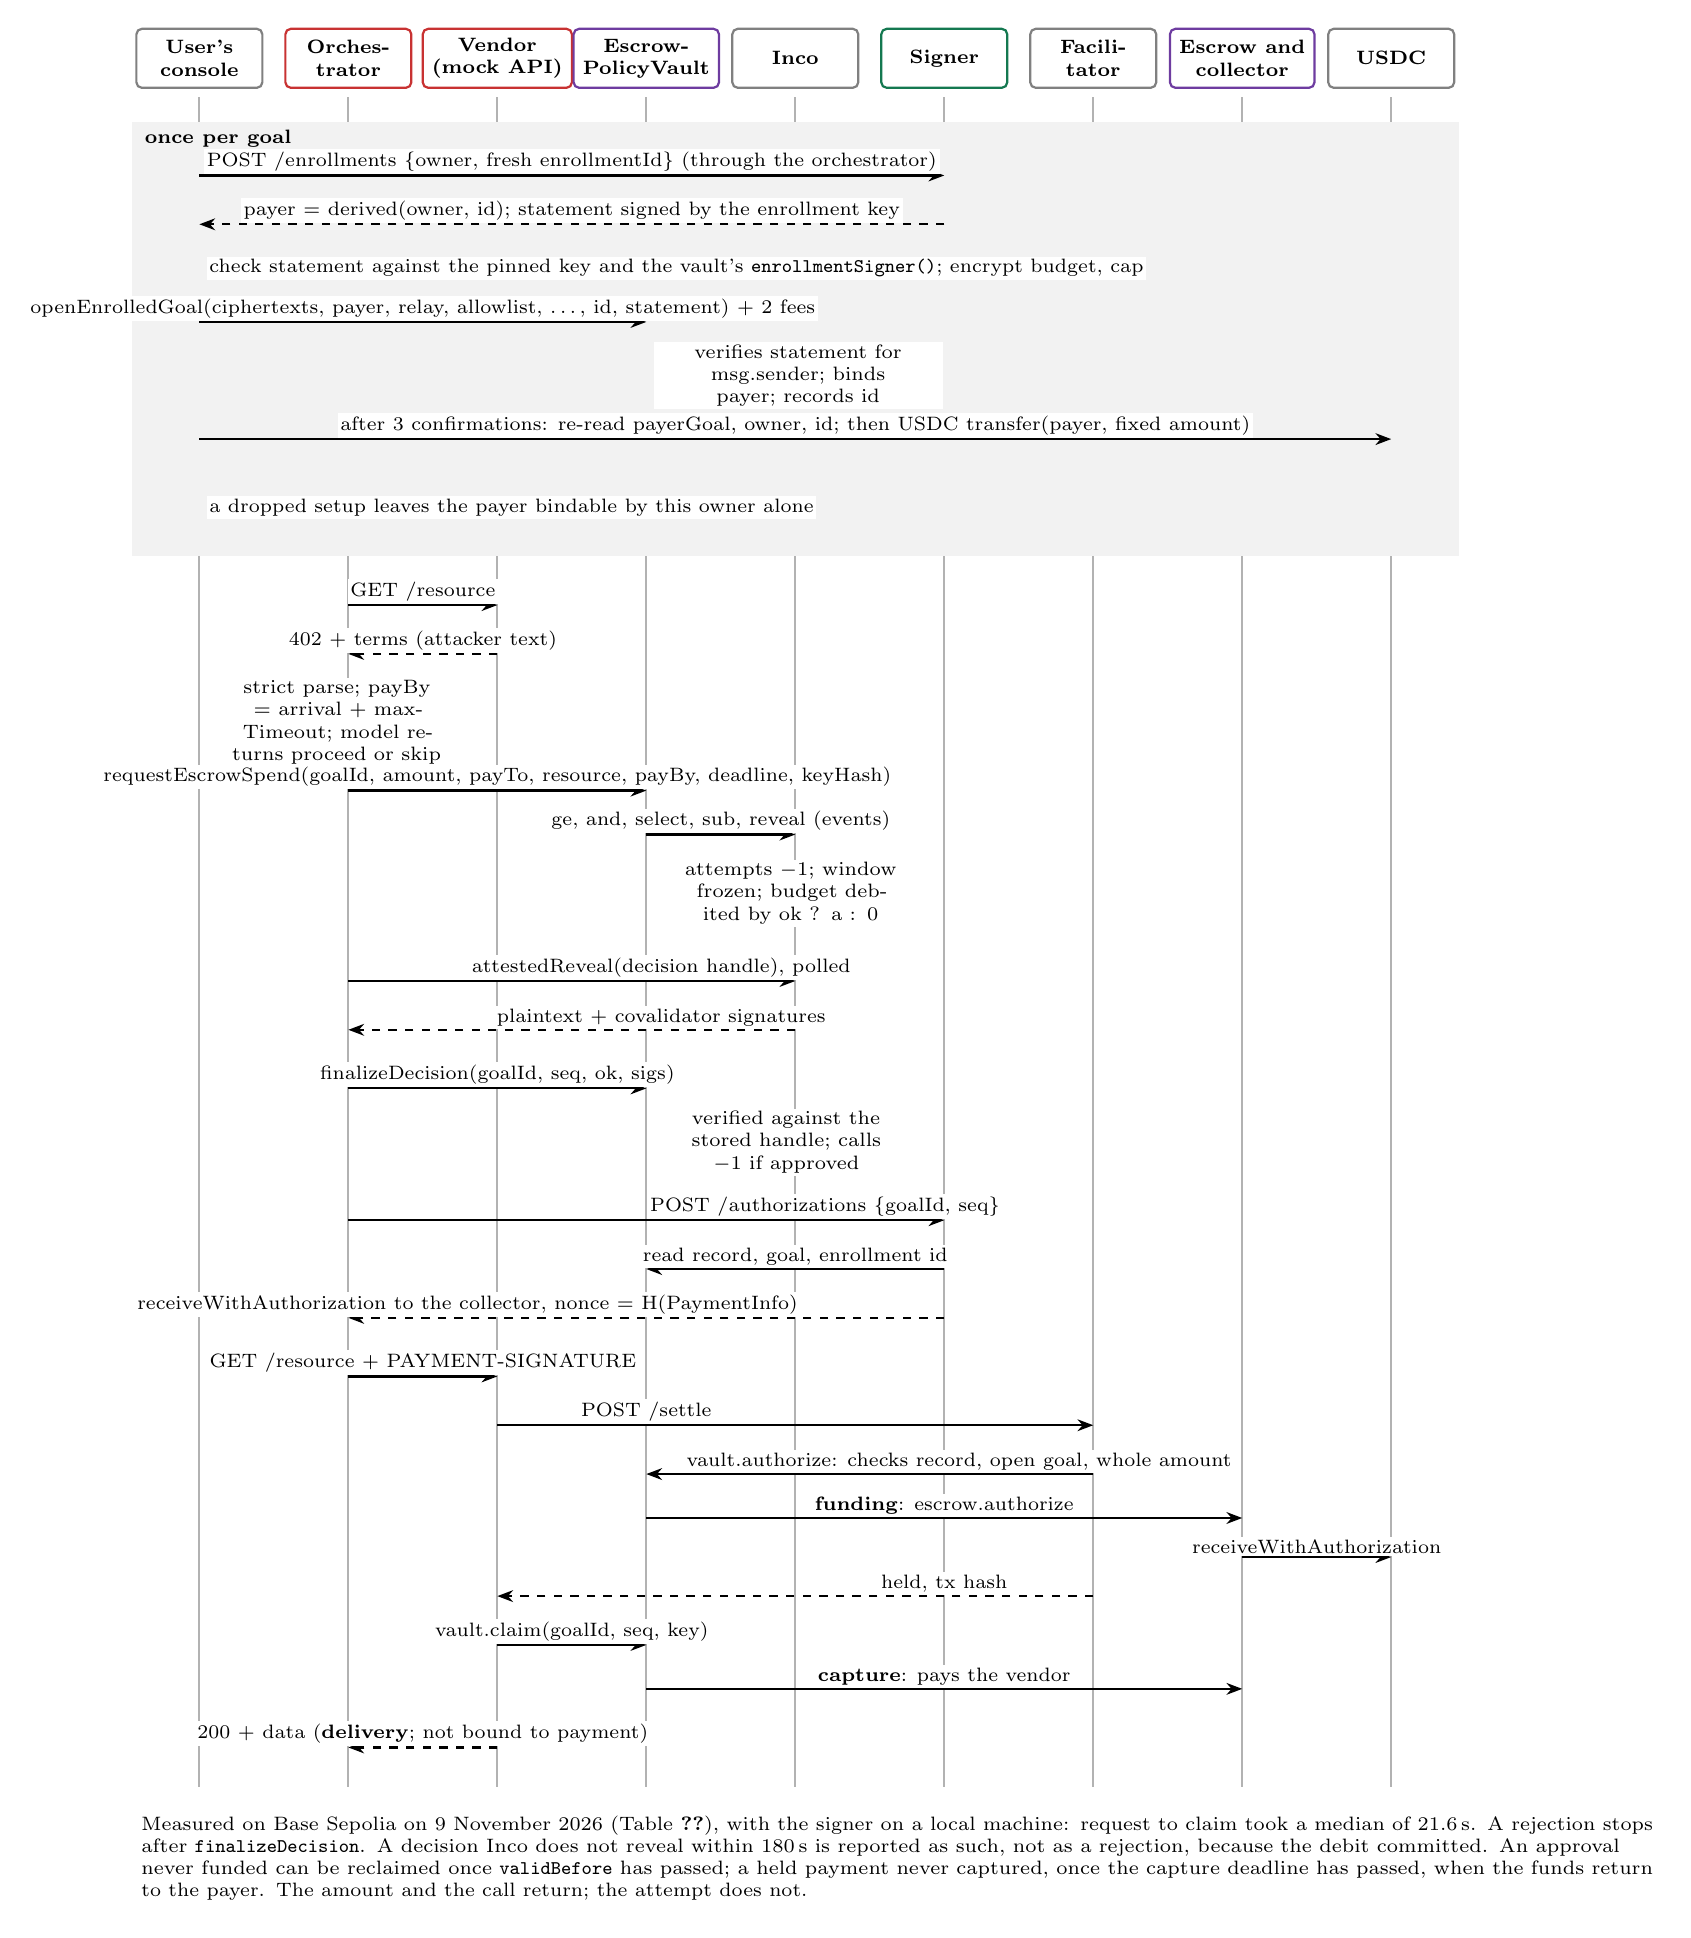
\begin{tikzpicture}[x=0.86cm,y=-0.62cm,
    msg/.style={-{Stealth[length=2mm]},thick},
    rmsg/.style={-{Stealth[length=2mm]},thick,dashed},
    mlab/.style={font=\scriptsize,fill=white,inner sep=1pt,align=center},
    act/.style={draw,thick,fill=white,font=\scriptsize\bfseries,align=center,minimum width=1.6cm,minimum height=0.75cm,rounded corners=2pt}]
  \def\xU{0}\def\xO{2.2}\def\xV{4.4}\def\xP{6.6}\def\xI{8.8}\def\xS{11.0}\def\xF{13.2}\def\xE{15.4}\def\xT{17.6}
  \node[act,draw=gray]      at (\xU,0) {User's\\console};
  \node[act,draw=untrusted] at (\xO,0) {Orches-\\trator};
  \node[act,draw=untrusted] at (\xV,0) {Vendor\\(mock API)};
  \node[act,draw=chain]     at (\xP,0) {Escrow-\\PolicyVault};
  \node[act,draw=gray]      at (\xI,0) {Inco};
  \node[act,draw=enclave]   at (\xS,0) {Signer};
  \node[act,draw=gray]      at (\xF,0) {Facili-\\tator};
  \node[act,draw=chain]     at (\xE,0) {Escrow and\\collector};
  \node[act,draw=gray]      at (\xT,0) {USDC};
  \foreach \x in {\xU,\xO,\xV,\xP,\xI,\xS,\xF,\xE,\xT} \draw[gray!60,thick] (\x,0.8) -- (\x,35.4);

  % --- setup
  \fill[gray!10] (-1,1.3) rectangle (18.6,10.2);
  \node[font=\scriptsize\bfseries,anchor=west] at (-0.95,1.65) {once per goal};
  \draw[msg] (\xU,2.4) -- node[mlab,above]{POST /enrollments \{owner, fresh enrollmentId\} (through the orchestrator)} (\xS,2.4);
  \draw[rmsg] (\xS,3.4) -- node[mlab,above]{payer = derived(owner, id); statement signed by the enrollment key} (\xU,3.4);
  \node[mlab,anchor=west] at (\xU+0.1,4.3) {check statement against the pinned key and the vault's \code{enrollmentSigner()}; encrypt budget, cap};
  \draw[msg] (\xU,5.4) -- node[mlab,above]{openEnrolledGoal(ciphertexts, payer, relay, allowlist, \ldots, id, statement) + 2 fees} (\xP,5.4);
  \node[mlab,anchor=west,text width=3.6cm] at (\xP+0.1,6.5) {verifies statement for msg.sender; binds payer; records id};
  \draw[msg] (\xU,7.8) -- node[mlab,above]{after 3 confirmations: re-read payerGoal, owner, id; then USDC transfer(payer, fixed amount)} (\xT,7.8);
  \node[mlab,anchor=west] at (\xU+0.1,9.2) {a dropped setup leaves the payer bindable by this owner alone};

  % --- run
  \draw[msg] (\xO,11.2) -- node[mlab,above]{GET /resource} (\xV,11.2);
  \draw[rmsg] (\xV,12.2) -- node[mlab,above]{402 + terms (attacker text)} (\xO,12.2);
  \node[mlab,anchor=west,text width=3.4cm] at (\xO-2.2,13.6) {strict parse; payBy = arrival + maxTimeout; model returns proceed or skip};
  \draw[msg] (\xO,15.0) -- node[mlab,above]{requestEscrowSpend(goalId, amount, payTo, resource, payBy, deadline, keyHash)} (\xP,15.0);
  \draw[msg] (\xP,15.9) -- node[mlab,above]{ge, and, select, sub, reveal (events)} (\xI,15.9);
  \node[mlab,anchor=west,text width=3.4cm] at (\xP+0.1,17.1) {attempts $-1$; window frozen; budget debited by ok ? a : 0};
  \draw[msg] (\xO,18.9) -- node[mlab,above,pos=0.7]{attestedReveal(decision handle), polled} (\xI,18.9);
  \draw[rmsg] (\xI,19.9) -- node[mlab,above,pos=0.3]{plaintext + covalidator signatures} (\xO,19.9);
  \draw[msg] (\xO,21.1) -- node[mlab,above]{finalizeDecision(goalId, seq, ok, sigs)} (\xP,21.1);
  \node[mlab,anchor=west,text width=3.3cm] at (\xP+0.1,22.2) {verified against the stored handle; calls $-1$ if approved};
  \draw[msg] (\xO,23.8) -- node[mlab,above,pos=0.8]{POST /authorizations \{goalId, seq\}} (\xS,23.8);
  \draw[msg] (\xS,24.8) -- node[mlab,above]{read record, goal, enrollment id} (\xP,24.8);
  \draw[rmsg] (\xS,25.8) -- node[mlab,above,pos=0.8]{receiveWithAuthorization to the collector, nonce = H(PaymentInfo)} (\xO,25.8);
  \draw[msg] (\xO,27.0) -- node[mlab,above]{GET /resource + PAYMENT-SIGNATURE} (\xV,27.0);
  \draw[msg] (\xV,28.0) -- node[mlab,above,pos=0.25]{POST /settle} (\xF,28.0);
  \draw[msg] (\xF,29.0) -- node[mlab,above,pos=0.3]{vault.authorize: checks record, open goal, whole amount} (\xP,29.0);
  \draw[msg] (\xP,29.9) -- node[mlab,above]{\textbf{funding}: escrow.authorize} (\xE,29.9);
  \draw[msg] (\xE,30.7) -- node[mlab,above]{receiveWithAuthorization} (\xT,30.7);
  \draw[rmsg] (\xF,31.5) -- node[mlab,above,pos=0.25]{held, tx hash} (\xV,31.5);
  \draw[msg] (\xV,32.5) -- node[mlab,above]{vault.claim(goalId, seq, key)} (\xP,32.5);
  \draw[msg] (\xP,33.4) -- node[mlab,above]{\textbf{capture}: pays the vendor} (\xE,33.4);
  \draw[rmsg] (\xV,34.6) -- node[mlab,above]{200 + data (\textbf{delivery}; not bound to payment)} (\xO,34.6);
  \node[font=\scriptsize,align=left,anchor=north west,text width=19.2cm] at (-1,35.8)
   {Measured on Base Sepolia on 9 November 2026 (Table~\ref{tab:baselines}), with the signer on a local machine: request to claim took a median of 21.6\,s. A rejection stops after \code{finalizeDecision}. A decision Inco does not reveal within 180\,s is reported as such, not as a rejection, because the debit committed. An approval never funded can be reclaimed once \code{validBefore} has passed; a held payment never captured, once the capture deadline has passed, when the funds return to the payer. The amount and the call return; the attempt does not.};
\end{tikzpicture}
}
\caption{One paid call, message by message, on the current design. Solid arrows are requests and dashed arrows responses; the grey band happens
once per goal. Funding, capture and delivery are separate steps.}
\label{fig:seq}
\end{figure*}

\end{document}
